\documentclass{article}
\usepackage{pgfplots}
\begin{document}
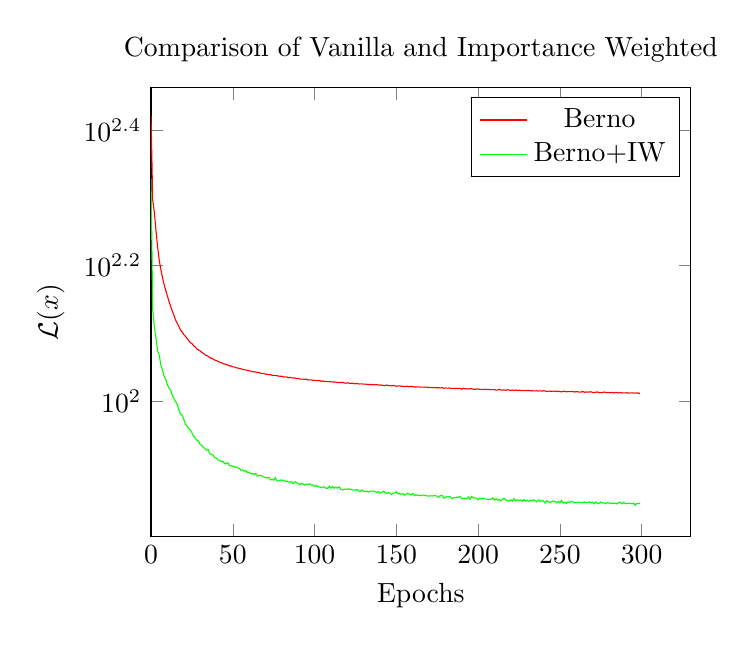
\begin{tikzpicture}\begin{semilogyaxis}    [title={Comparison of Vanilla and Importance Weighted},    xlabel={Epochs},ylabel={$\mathcal{L}(x)$},    xmin=0.0, xmax=330.0,ymin=63.1280970653, ymax=290.302163696,]    \addplot[color=red,]    coordinates {(0,263.911057906)(1,198.213255227)(2,190.304746094)(3,178.87626487)(4,169.086181335)(5,161.527062711)(6,156.384731972)(7,152.215601612)(8,148.611141996)(9,145.638506608)(10,142.924132968)(11,140.344120636)(12,137.979534649)(13,135.770691209)(14,133.905019739)(15,131.752419739)(16,130.218475314)(17,128.896445618)(18,127.414261669)(19,126.477938871)(20,125.370981806)(21,124.637320931)(22,123.725098253)(23,122.82003633)(24,121.97621564)(25,121.58177733)(26,120.742236287)(27,120.238140037)(28,119.374420554)(29,119.023158972)(30,118.607805509)(31,118.065131212)(32,117.60139052)(33,117.004031622)(34,116.718400712)(35,116.41280125)(36,115.757396102)(37,115.78068358)(38,115.311512451)(39,114.938878132)(40,114.766606986)(41,114.397145122)(42,114.068754716)(43,113.958563232)(44,113.586094263)(45,113.409035561)(46,113.245632921)(47,112.991837852)(48,112.665145236)(49,112.659438712)(50,112.346413921)(51,112.275464713)(52,111.965743034)(53,111.909392631)(54,111.668662997)(55,111.587927884)(56,111.359355261)(57,111.197885062)(58,111.16540107)(59,110.941213629)(60,110.819788527)(61,110.707621737)(62,110.529289024)(63,110.37031558)(64,110.406151165)(65,110.126960144)(66,110.205561454)(67,109.840602986)(68,109.876750807)(69,109.761879716)(70,109.585940247)(71,109.505338482)(72,109.363434989)(73,109.430629342)(74,109.109307736)(75,109.116950628)(76,109.086401492)(77,108.97200463)(78,108.851236808)(79,108.78205479)(80,108.765222321)(81,108.507579249)(82,108.57878135)(83,108.516908292)(84,108.210548054)(85,108.397520225)(86,108.204046173)(87,108.158662775)(88,108.119251099)(89,107.944731265)(90,108.016901661)(91,107.73954816)(92,107.710474063)(93,107.722989225)(94,107.645931951)(95,107.707727384)(96,107.39834155)(97,107.476644176)(98,107.438700867)(99,107.269752627)(100,107.226178214)(101,107.27347143)(102,107.135012554)(103,107.281838046)(104,106.898756478)(105,107.094956707)(106,106.842869887)(107,106.930941065)(108,106.833211892)(109,106.811454052)(110,106.74715787)(111,106.697943781)(112,106.671509316)(113,106.647949122)(114,106.467280981)(115,106.508278073)(116,106.494360435)(117,106.514126157)(118,106.379689359)(119,106.226369046)(120,106.389516629)(121,106.264832902)(122,106.141597665)(123,106.29064829)(124,106.089729767)(125,106.044406197)(126,106.192846985)(127,105.948057792)(128,106.009500122)(129,105.998451857)(130,105.889937189)(131,105.930427121)(132,105.831874473)(133,105.746641471)(134,105.81172312)(135,105.682832489)(136,105.784496613)(137,105.645301098)(138,105.740606662)(139,105.552423151)(140,105.615537886)(141,105.549215324)(142,105.395384771)(143,105.389573253)(144,105.572810267)(145,105.387793316)(146,105.453733201)(147,105.254012659)(148,105.439921903)(149,105.314982494)(150,105.142971275)(151,105.266738933)(152,105.306561043)(153,105.18495611)(154,105.064412842)(155,105.095941134)(156,105.06192129)(157,105.141722329)(158,104.962899822)(159,105.14358096)(160,104.997266513)(161,104.893339261)(162,104.877855197)(163,104.918052826)(164,104.899852669)(165,104.81209481)(166,104.848601851)(167,104.805977284)(168,104.821523576)(169,104.803668463)(170,104.667991735)(171,104.766617543)(172,104.629148407)(173,104.700370983)(174,104.605317577)(175,104.63054005)(176,104.611541415)(177,104.561938019)(178,104.629640406)(179,104.441594585)(180,104.512454348)(181,104.45640908)(182,104.514999376)(183,104.452973189)(184,104.380399669)(185,104.375079595)(186,104.317090399)(187,104.428788841)(188,104.330876146)(189,104.386269698)(190,104.100571511)(191,104.423475272)(192,104.240891294)(193,104.259876778)(194,104.166290921)(195,104.302629908)(196,104.255080955)(197,104.077226341)(198,104.0614371)(199,104.126844025)(200,104.175664645)(201,104.05645462)(202,104.047560023)(203,103.987927413)(204,104.079551905)(205,103.982308322)(206,104.042302163)(207,103.970290777)(208,103.958484331)(209,103.947987879)(210,103.96327172)(211,103.76637422)(212,103.808471305)(213,104.091310647)(214,103.776604892)(215,103.799186332)(216,103.860700254)(217,103.682867903)(218,103.907387848)(219,103.812983232)(220,103.614567913)(221,103.836631248)(222,103.59787495)(223,103.838682875)(224,103.65001125)(225,103.76185207)(226,103.608184717)(227,103.631562625)(228,103.600637956)(229,103.59588716)(230,103.617301331)(231,103.645032404)(232,103.505390778)(233,103.568912243)(234,103.512093561)(235,103.475622905)(236,103.542617298)(237,103.458997664)(238,103.525815666)(239,103.391191656)(240,103.57085022)(241,103.501735021)(242,103.269330347)(243,103.432664781)(244,103.366980355)(245,103.361040011)(246,103.434469188)(247,103.279656011)(248,103.424536896)(249,103.280434931)(250,103.293235501)(251,103.138385315)(252,103.381104029)(253,103.340434723)(254,103.193569599)(255,103.243596954)(256,103.220414692)(257,103.283062328)(258,103.251557936)(259,103.102934931)(260,103.248284232)(261,103.181984031)(262,103.060927512)(263,103.05878762)(264,103.356516363)(265,102.997390858)(266,103.102375141)(267,103.061714866)(268,103.104844236)(269,103.193875705)(270,102.934247242)(271,102.966972268)(272,103.023014429)(273,103.135971902)(274,102.914399802)(275,102.884195876)(276,102.911637296)(277,103.110926569)(278,102.980401265)(279,102.88293611)(280,102.968769601)(281,102.855491666)(282,102.971831748)(283,102.752470301)(284,102.950700476)(285,102.961044977)(286,102.733744424)(287,102.971840598)(288,102.765343822)(289,102.825684038)(290,102.796692491)(291,102.862699835)(292,102.688350164)(293,102.817591525)(294,102.802225425)(295,102.750529341)(296,102.698477298)(297,102.824272738)(298,102.667397516)(299,102.672452365)    };    \addplot[color=green,]    coordinates {(0,212.889503881)(1,136.69067473)(2,128.82833134)(3,124.040854936)(4,118.690849804)(5,116.909000924)(6,113.013927626)(7,111.075254586)(8,108.798369917)(9,107.562806091)(10,105.667284851)(11,104.449745872)(12,103.738867798)(13,101.913222407)(14,100.880470165)(15,99.7707582092)(16,98.9113952359)(17,96.9467745001)(18,95.6420740024)(19,95.3488831676)(20,93.9665334251)(21,92.4877756431)(22,91.8431637018)(23,91.0363048068)(24,90.5232136397)(25,89.7399208069)(26,88.7281854803)(27,88.1798480225)(28,87.5367355208)(29,87.3209809875)(30,86.2576438349)(31,86.0276815102)(32,85.4221434021)(33,85.0303677923)(34,84.5800309337)(35,84.7152453891)(36,83.5131790022)(37,83.4104959453)(38,83.1304513758)(39,82.4841615989)(40,82.3764996546)(41,81.7875932936)(42,81.7060721588)(43,81.3806930681)(44,81.4111268546)(45,80.838586731)(46,80.7406091725)(47,81.017188041)(48,80.2124638228)(49,80.2271451361)(50,80.0896083138)(51,79.8871128637)(52,79.8942684867)(53,79.7550364408)(54,79.538298645)(55,79.0118305414)(56,79.0969413133)(57,78.7534699735)(58,78.9117192979)(59,78.3776827171)(60,78.4891304779)(61,78.0464635398)(62,78.1325949721)(63,77.9003106967)(64,78.1739014712)(65,77.4500395133)(66,77.6281871865)(67,77.6110464131)(68,77.474847426)(69,77.2124328683)(70,77.1030504678)(71,76.9742827121)(72,77.1269824912)(73,76.453514002)(74,76.6268032559)(75,76.3920169484)(76,77.0279490245)(77,76.1911592518)(78,76.1912690319)(79,76.4120253546)(80,76.3616653512)(81,76.4200014773)(82,76.1013489741)(83,76.1299544941)(84,75.9456712133)(85,75.8474544456)(86,75.9958151453)(87,75.4516047114)(88,75.9606080211)(89,75.7825870514)(90,75.4166851807)(91,75.2730201028)(92,75.5633785178)(93,75.3926641221)(94,75.1231771504)(95,75.3425059509)(96,75.2793357017)(97,75.42107236)(98,75.0752778209)(99,75.1563735268)(100,74.7741940308)(101,75.0860549094)(102,74.687021852)(103,74.6451232633)(104,74.4814327032)(105,74.6204650948)(106,74.6206243688)(107,74.3239216544)(108,74.2764617642)(109,74.8516898277)(110,74.3182112052)(111,74.7670684121)(112,74.3290488018)(113,74.5695130088)(114,74.3323224362)(115,74.6895237246)(116,74.0510518993)(117,73.9067425815)(118,74.0074700442)(119,74.1338988495)(120,74.0175181926)(121,74.1761847895)(122,74.0235229562)(123,73.9181140345)(124,73.8457655473)(125,73.8702288749)(126,74.0162856362)(127,73.6437659316)(128,73.4565949943)(129,73.9170945116)(130,73.5467081313)(131,73.4937463864)(132,73.5905630146)(133,73.353295621)(134,73.6264864766)(135,73.5908654092)(136,73.5732003923)(137,73.4532649994)(138,73.2716727794)(139,73.465524188)(140,73.112097598)(141,73.2420930204)(142,73.5635126287)(143,73.3090762398)(144,72.9897125105)(145,73.2172430489)(146,73.1516952931)(147,72.7228497869)(148,73.0782187098)(149,73.1016768508)(150,73.4024589885)(151,72.880766879)(152,73.0312317588)(153,72.7873863844)(154,72.9423721105)(155,72.5628787509)(156,72.8360966284)(157,73.047174426)(158,72.8167339325)(159,72.6396780465)(160,73.0304298262)(161,72.4665298601)(162,72.6912430434)(163,72.5760772358)(164,72.4846100339)(165,72.459022411)(166,72.5838312045)(167,72.6003749293)(168,72.5145784413)(169,72.3569016474)(170,72.3737294076)(171,72.4213695249)(172,72.3710491943)(173,72.4755430534)(174,72.4657969249)(175,72.2095316592)(176,72.0375349288)(177,72.5440174311)(178,72.5334384502)(179,71.8655854936)(180,72.008425508)(181,72.254446425)(182,72.1637018724)(183,72.2237791096)(184,71.714810257)(185,71.9142984702)(186,72.0176052856)(187,72.0815261771)(188,72.0838776606)(189,72.2727386128)(190,71.688610285)(191,71.8585383883)(192,71.8177259757)(193,71.7062380357)(194,72.1454219471)(195,71.6026708776)(196,72.2864398055)(197,71.9247254597)(198,71.868394928)(199,71.8450078375)(200,71.4535544239)(201,71.8534567261)(202,71.670494683)(203,71.8755769626)(204,71.7016650391)(205,71.6363452565)(206,71.504623205)(207,71.5315711698)(208,71.587473741)(209,71.8978508828)(210,71.4103687564)(211,71.70563883)(212,71.3756308677)(213,71.5474994174)(214,71.1844528337)(215,71.60504733)(216,71.8060398934)(217,71.4310690862)(218,71.3169561282)(219,71.1020025912)(220,71.425415476)(221,71.1148356559)(222,71.7071190435)(223,71.1754220234)(224,71.483830067)(225,71.261985321)(226,71.4267416937)(227,71.0780576116)(228,71.5027765656)(229,71.1248665203)(230,71.3434074541)(231,71.0519401204)(232,71.3568696039)(233,71.2187969555)(234,71.4516134782)(235,71.2335008032)(236,70.9221232674)(237,71.3969466123)(238,70.9965213568)(239,71.3100876895)(240,71.1295058164)(241,70.6539552723)(242,71.2394960577)(243,70.9955520907)(244,70.8132880679)(245,71.0490945296)(246,71.1247871052)(247,71.0870736417)(248,70.7841236739)(249,70.9903914504)(250,70.7095126967)(251,71.2655674189)(252,70.6899923706)(253,70.8693695623)(254,70.6116099063)(255,70.951697138)(256,70.8354414368)(257,71.0545902252)(258,70.8714400898)(259,70.8538174022)(260,70.822078039)(261,70.8707302163)(262,70.8950232905)(263,70.7760084395)(264,70.7706362083)(265,70.9704128127)(266,70.7572787822)(267,70.7819294947)(268,70.9383078766)(269,70.7281015916)(270,70.8945835599)(271,70.482622972)(272,70.93528905)(273,70.5277008334)(274,70.5941716211)(275,70.8907409599)(276,70.6606239388)(277,70.7143197632)(278,70.4889673545)(279,70.7734613106)(280,70.716083048)(281,70.5357097002)(282,70.6280721283)(283,70.5701076577)(284,70.6263676938)(285,70.4352469635)(286,70.7839288816)(287,70.8557285656)(288,70.4485128229)(289,70.8420001637)(290,70.5595037981)(291,70.5228122572)(292,70.6055964106)(293,70.5968888716)(294,70.4848312725)(295,70.6190093855)(296,70.1423300726)(297,70.5032779763)(298,70.5609679066)(299,70.6179385029)    };    \legend{Berno,Berno+IW,}\end{semilogyaxis}\end{tikzpicture}\\
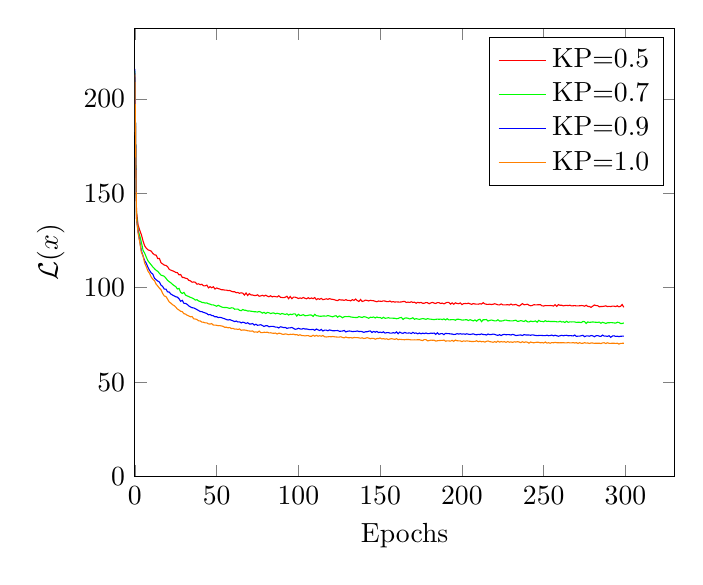
\begin{tikzpicture}\begin{axis}    [% title={Comparison of Dropout Values for Cost},
    xlabel={Epochs},ylabel={$\mathcal{L}(x)$},    xmin=0, xmax=330.0,ymin=0, ymax=237.42232074,]    \addplot[color=red,]    coordinates {(0,213.611983948)(1,140.18732924)(2,133.135610338)(3,130.399719419)(4,128.024808128)(5,124.77403889)(6,122.163706984)(7,120.90422957)(8,120.05607261)(9,119.76171979)(10,119.383919553)(11,118.175268471)(12,117.429623926)(13,117.256619942)(14,115.439550171)(15,115.510523349)(16,113.219375999)(17,112.620345778)(18,111.956657743)(19,111.793498119)(20,111.171441068)(21,109.736893394)(22,109.28692971)(23,108.983262926)(24,108.627620766)(25,108.098348514)(26,107.976467465)(27,106.807655445)(28,106.991383459)(29,105.44258452)(30,105.402134621)(31,105.004501038)(32,104.813612477)(33,103.91330959)(34,103.645676589)(35,102.91079655)(36,103.053433366)(37,102.866839794)(38,101.852876878)(39,102.072165902)(40,101.607229018)(41,101.820079332)(42,101.035628343)(43,100.962292744)(44,101.387939828)(45,99.9537455333)(46,100.543978715)(47,99.9916471447)(48,100.493672666)(49,99.306105957)(50,99.8871899969)(51,99.5275249412)(52,99.2779960077)(53,98.9154440585)(54,98.9101204057)(55,98.733694139)(56,98.728449277)(57,98.461963931)(58,98.5245701738)(59,98.1555898909)(60,97.8545828802)(61,97.8821508095)(62,97.3483742454)(63,97.4739813787)(64,97.0512139754)(65,97.3083419939)(66,97.1000620339)(67,96.1211658131)(68,97.222053944)(69,95.8810383051)(70,96.8617865268)(71,96.1876468589)(72,96.1277068953)(73,95.903643244)(74,95.8516946272)(75,96.2546559282)(76,95.4969988043)(77,95.6693305969)(78,95.990305148)(79,95.5831520497)(80,96.0392578541)(81,95.5534802801)(82,95.2042282104)(83,95.7647049644)(84,95.1364231873)(85,95.4236530928)(86,95.2903656145)(87,95.1127528936)(88,95.7217718922)(89,94.9602949524)(90,94.8110238231)(91,94.7296563721)(92,94.9764315518)(93,95.468109658)(94,94.1866127985)(95,95.3313384316)(96,94.1990991072)(97,95.0039223688)(98,94.9899989596)(99,94.7225640453)(100,94.2842888017)(101,94.6004848966)(102,94.3207508989)(103,94.8157336703)(104,94.4017254639)(105,94.1065885648)(106,94.7126369962)(107,94.1927085322)(108,94.5917877059)(109,94.1949142733)(110,94.7765461592)(111,93.6764934332)(112,94.189502078)(113,93.8595896357)(114,94.3427665572)(115,93.6743502391)(116,93.8669215809)(117,94.1364919489)(118,93.8388804072)(119,94.2113019215)(120,93.9383510104)(121,93.8336909069)(122,93.6571312089)(123,93.3188643299)(124,93.1457136536)(125,93.7332522583)(126,93.4874144259)(127,93.524207403)(128,93.2823169084)(129,93.6898468572)(130,93.3077062572)(131,93.3324563599)(132,93.0280900296)(133,93.6728287714)(134,93.2696682601)(135,94.0037447843)(136,93.2077322665)(137,92.7058163452)(138,93.7697184892)(139,92.7220354808)(140,92.9681773931)(141,93.4360756337)(142,93.2726210161)(143,92.9897828536)(144,93.3417346469)(145,93.1581353066)(146,93.0993127441)(147,92.7975571372)(148,92.5549210566)(149,92.9567054332)(150,92.8302947166)(151,92.7592158508)(152,93.0528797774)(153,92.9330664062)(154,92.6696998596)(155,92.6318971391)(156,92.9723107355)(157,92.4377223899)(158,92.6380902516)(159,92.3792817827)(160,92.5151450833)(161,92.424616616)(162,92.38853972)(163,92.4709234619)(164,92.6907117532)(165,92.7555661843)(166,92.1862243652)(167,92.3680494135)(168,92.2127138311)(169,92.5590900352)(170,92.20048215)(171,92.342269731)(172,91.7910020585)(173,92.2500653354)(174,92.0132443237)(175,92.2266598095)(176,91.7797974465)(177,91.8020800365)(178,92.1568803267)(179,92.0421813133)(180,91.510495439)(181,91.9553103915)(182,92.2301329595)(183,91.8426958258)(184,91.6622891235)(185,92.1257831782)(186,92.0898311129)(187,91.6649375777)(188,91.869218861)(189,91.4809727131)(190,91.903315499)(191,92.2579885309)(192,92.2335494718)(193,91.2896772073)(194,91.9680852647)(195,91.2646139249)(196,91.9935879794)(197,91.6474140375)(198,91.531919736)(199,91.9635053947)(200,91.0681544217)(201,91.5510597506)(202,91.651471405)(203,91.5496334284)(204,91.826006442)(205,91.4640564936)(206,91.2044036727)(207,91.6090379195)(208,91.3583173578)(209,91.3294433871)(210,91.2666262817)(211,91.52830848)(212,91.3455044001)(213,92.0741345215)(214,91.455580486)(215,91.2313515958)(216,91.1773025097)(217,91.3149301009)(218,91.0836041676)(219,91.2343638333)(220,91.5038699063)(221,91.2759326449)(222,90.9520749734)(223,90.881909471)(224,91.431077645)(225,90.9361196067)(226,90.8855583191)(227,90.9350551813)(228,91.0358515306)(229,90.8197500749)(230,91.366390797)(231,90.8742534846)(232,90.9825250244)(233,91.1631697915)(234,90.6874451516)(235,90.3214517212)(236,90.8902434748)(237,91.5779855624)(238,91.0027242487)(239,91.016811468)(240,91.2977366638)(241,90.739137927)(242,90.4453065629)(243,90.584449449)(244,91.0086730541)(245,90.9174829379)(246,90.9476875097)(247,90.9791460072)(248,91.0291654968)(249,90.407079981)(250,90.3193673429)(251,90.5547389637)(252,90.4821096594)(253,90.4856060791)(254,90.5668820745)(255,90.5008590005)(256,90.3156455161)(257,91.0098980297)(258,90.1034014476)(259,91.0529214061)(260,90.6726082819)(261,90.7373472456)(262,90.388000516)(263,90.5852433291)(264,90.6458044711)(265,90.5188269737)(266,90.7493088462)(267,90.3724605352)(268,90.4386719721)(269,90.5193221352)(270,90.3576756009)(271,90.4086131425)(272,90.4292802707)(273,90.569722831)(274,90.4777214883)(275,90.215136691)(276,90.7068161982)(277,90.0946172263)(278,90.0319270463)(279,89.6243378587)(280,90.2400622697)(281,90.8546568714)(282,90.5377965338)(283,90.5013866216)(284,89.8489982605)(285,90.0823363009)(286,90.0735631214)(287,90.2040368514)(288,90.4084086331)(289,90.0001905684)(290,90.1478595664)(291,89.9958828458)(292,90.2765512779)(293,90.2110899492)(294,90.0210393177)(295,90.4161890203)(296,89.8837258495)(297,90.1795156583)(298,91.0725844782)(299,89.6297112482)    };    \addplot[color=green,]    coordinates {(0,214.870156652)(1,138.420214095)(2,130.315231947)(3,127.553233823)(4,123.974801955)(5,119.829264374)(6,118.279018485)(7,116.152291773)(8,114.246067061)(9,113.159955805)(10,112.061284582)(11,110.999344677)(12,110.061311909)(13,109.214917006)(14,108.661174913)(15,107.652753518)(16,106.642363892)(17,106.411822843)(18,106.020106173)(19,105.040679973)(20,103.885582678)(21,103.184375499)(22,102.599161113)(23,101.801667231)(24,101.099923706)(25,100.620336553)(26,99.314928464)(27,99.6515905207)(28,97.6019067799)(29,96.9577655723)(30,97.5208233088)(31,96.0611297053)(32,95.675633101)(33,95.3081980619)(34,94.8892831143)(35,94.5714155995)(36,94.1128608426)(37,93.4403350136)(38,93.6682945668)(39,92.9367888295)(40,92.7338731107)(41,92.2090962358)(42,92.1613211198)(43,91.837235149)(44,91.9705283286)(45,91.4814981634)(46,91.3199196972)(47,90.9048228732)(48,90.8977095448)(49,90.5602925457)(50,90.1892748607)(51,90.7127239019)(52,90.2337749273)(53,89.8098288796)(54,89.5695165599)(55,89.4958905307)(56,89.5028270791)(57,89.3190107172)(58,89.0481610246)(59,89.3632296475)(60,89.2784141818)(61,88.6192438854)(62,88.6589732638)(63,88.7007866461)(64,88.0385941245)(65,87.8257203258)(66,88.4583539928)(67,88.0963810453)(68,88.0337612638)(69,87.6306257213)(70,87.7301812397)(71,87.5399717019)(72,87.4496276578)(73,87.2786976485)(74,87.2426797347)(75,87.1320374645)(76,87.3923365506)(77,87.0941870533)(78,86.5277147536)(79,86.9653163563)(80,86.3338212724)(81,86.8822792469)(82,86.7573875289)(83,86.3184753834)(84,86.574380077)(85,86.6500987521)(86,86.1874647245)(87,86.4851209606)(88,86.268961251)(89,85.9376861988)(90,86.3794110177)(91,86.0784655762)(92,85.8549691148)(93,86.2014910611)(94,85.5127039268)(95,86.0103405762)(96,85.7376453261)(97,86.1322527383)(98,86.166138916)(99,85.0102442516)(100,85.927780082)(101,85.2759978485)(102,85.437036216)(103,85.7228837724)(104,85.1629249295)(105,85.2067716286)(106,85.4069564403)(107,85.5510473841)(108,85.5207710405)(109,84.7946066978)(110,85.9130314428)(111,85.2192742504)(112,85.072487467)(113,84.9142251518)(114,84.8860689614)(115,85.0248310158)(116,85.0069939006)(117,84.9390543296)(118,85.2528283275)(119,85.0660427163)(120,84.8037571023)(121,84.5885448525)(122,84.9765426636)(123,85.1708403986)(124,84.3796697443)(125,85.0553857422)(126,84.7108572457)(127,84.0782047341)(128,84.629805173)(129,84.7332257635)(130,84.6919879428)(131,84.7927964713)(132,84.5007958568)(133,84.3884010176)(134,84.3051656203)(135,84.2271676983)(136,84.2038112155)(137,84.6991061609)(138,84.458704071)(139,84.2341667037)(140,84.6478091153)(141,84.5471891785)(142,84.1950016369)(143,83.8179136242)(144,84.3808906)(145,84.2535355793)(146,84.4977275294)(147,83.972999975)(148,84.4763268072)(149,84.1389602661)(150,84.2236982796)(151,83.7183624545)(152,84.3385676644)(153,83.8259258201)(154,83.8846010104)(155,84.1316794933)(156,83.888755084)(157,83.9322339006)(158,83.8413687966)(159,83.7921620594)(160,83.5728130479)(161,83.701048688)(162,84.0920168443)(163,84.2539291382)(164,83.2122543058)(165,83.8750032806)(166,84.0060123652)(167,83.8260972456)(168,83.4689268008)(169,83.6796035697)(170,84.0763642467)(171,83.2972594105)(172,83.6004581243)(173,83.4242536094)(174,83.2409453375)(175,83.4722192313)(176,83.6706313532)(177,83.5025942854)(178,83.2477314134)(179,83.6391253662)(180,83.4178883778)(181,83.332330239)(182,83.2076757604)(183,83.1160052282)(184,83.2571568853)(185,83.3735539384)(186,83.2770165808)(187,83.3971421883)(188,83.0843249789)(189,83.4894906894)(190,82.9381799733)(191,83.5756591173)(192,82.9672124551)(193,83.0144879428)(194,83.125135068)(195,83.1003886691)(196,82.7854520971)(197,83.3359429585)(198,83.3011672974)(199,83.1368656436)(200,82.8596509552)(201,82.9010264518)(202,83.016791035)(203,83.0334751615)(204,82.6239663696)(205,83.0672074197)(206,82.7639159047)(207,82.4296782754)(208,82.9318576743)(209,82.2945258123)(210,83.0302327798)(211,83.3258488464)(212,82.0435404136)(213,83.031598483)(214,83.0513703502)(215,83.1511381669)(216,82.3436374595)(217,82.7023922938)(218,82.8849622761)(219,82.7083120728)(220,82.4307899267)(221,82.4616999262)(222,83.0405185491)(223,82.3669166288)(224,82.3789618059)(225,82.4347757444)(226,82.7899948814)(227,82.8630497048)(228,82.5685464686)(229,82.5046944219)(230,82.4130984913)(231,82.4182261935)(232,82.6288097867)(233,82.7867598239)(234,82.1713951458)(235,82.2963935921)(236,82.5854754084)(237,82.3608812852)(238,82.1169823941)(239,82.7027742906)(240,81.9885283383)(241,81.8623723949)(242,82.3280506758)(243,82.1132123635)(244,82.1446518985)(245,82.4041611689)(246,81.730336921)(247,82.7179852572)(248,82.204655727)(249,82.1710944991)(250,81.9829544275)(251,82.5484273806)(252,82.1093899397)(253,82.2901089616)(254,82.0798798578)(255,82.125348594)(256,82.1261571295)(257,82.0775339092)(258,81.9534230666)(259,81.8953144073)(260,82.2463850958)(261,81.8480450856)(262,81.9826956732)(263,81.5991771559)(264,82.2231609969)(265,81.6801091073)(266,81.9156964874)(267,81.8692735707)(268,81.8999719169)(269,81.8809726507)(270,81.6320365975)(271,81.7119881647)(272,81.6863255449)(273,81.5094223855)(274,82.1497115118)(275,82.0475640522)(276,81.0604660242)(277,81.8864986281)(278,81.6382845584)(279,81.7427749634)(280,81.8848708344)(281,81.7607927288)(282,81.693744056)(283,81.6574710707)(284,81.7957428395)(285,81.2024236852)(286,81.6864437589)(287,81.3977075334)(288,81.0720703819)(289,81.4265607938)(290,81.4371619277)(291,81.5132896146)(292,81.4836809679)(293,81.3571913979)(294,81.2487156816)(295,81.7022625178)(296,81.6577165708)(297,81.0779968123)(298,81.0718599285)(299,81.3702291454)    };    \addplot[color=blue,]    coordinates {(0,215.8384734)(1,136.601483931)(2,129.551664581)(3,124.607109153)(4,119.507357039)(5,116.815960347)(6,114.296949837)(7,112.912589361)(8,110.834768843)(9,109.116878662)(10,107.886004417)(11,107.172197904)(12,104.991113059)(13,104.257106656)(14,103.54942423)(15,102.999477747)(16,101.365754991)(17,100.657033067)(18,99.2550544739)(19,99.2633755216)(20,97.7858544506)(21,97.7082407032)(22,96.6407129739)(23,96.1362954712)(24,95.6980433932)(25,95.2148625461)(26,94.9999545843)(27,94.1665171259)(28,92.8140341603)(29,93.3106960643)(30,91.7495737804)(31,91.6977600098)(32,91.1752568332)(33,90.3614225353)(34,89.8406413963)(35,89.4045970709)(36,89.3060914889)(37,88.8682864935)(38,88.4041238681)(39,87.9086160556)(40,87.386510523)(41,87.3167237993)(42,86.9224127336)(43,86.6690864286)(44,86.3129240695)(45,85.6614154746)(46,85.8049856637)(47,85.2891301381)(48,85.1388681585)(49,84.5862819602)(50,84.6716788899)(51,84.1565041559)(52,84.3345454545)(53,84.0981897597)(54,83.8006549766)(55,83.5357553794)(56,83.1469325811)(57,82.9030120433)(58,83.0990911727)(59,82.7674890414)(60,82.4494290508)(61,82.0324814675)(62,82.3602942241)(63,81.8624638367)(64,81.9340980946)(65,81.3610738858)(66,81.7546448794)(67,81.5319767414)(68,81.0829956748)(69,81.4568557947)(70,80.7872998949)(71,80.7628709897)(72,81.0154140056)(73,80.2121364524)(74,80.6536714658)(75,80.1008480349)(76,80.2213746088)(77,80.4128141923)(78,79.9552653018)(79,79.5071927435)(80,79.8779327531)(81,79.8933596247)(82,79.3004967846)(83,79.4916309149)(84,79.5180192843)(85,79.4663571236)(86,79.1174646204)(87,79.1366321356)(88,78.7105505718)(89,79.2976636783)(90,79.1434709722)(91,78.8703263023)(92,78.9534567816)(93,78.46615156)(94,78.6947441379)(95,78.7250775077)(96,78.9793949266)(97,78.4669803134)(98,77.994704465)(99,78.1328830095)(100,78.5208978063)(101,78.2063856645)(102,78.0481426933)(103,78.3872793232)(104,78.134710943)(105,78.1563891324)(106,77.9635571775)(107,77.7863358584)(108,77.8491326211)(109,77.9385080095)(110,77.4537812805)(111,78.1566911247)(112,77.6900423154)(113,77.3340005354)(114,77.9309584115)(115,77.0592485671)(116,77.5287978155)(117,77.546876297)(118,77.2230330172)(119,77.6581750766)(120,77.4287545222)(121,77.1791651778)(122,77.2324570673)(123,77.2498461498)(124,77.3415248593)(125,76.958931212)(126,76.973895985)(127,77.0761110895)(128,77.372790021)(129,76.5930095118)(130,76.9076765303)(131,77.0787751839)(132,77.0084970093)(133,76.72747028)(134,76.8654086997)(135,76.8800515955)(136,77.1016694641)(137,76.7946580852)(138,76.8717832392)(139,76.7355181815)(140,76.3448611311)(141,76.6535278806)(142,76.6900183452)(143,76.9718477492)(144,77.1226234436)(145,76.3046080364)(146,76.849566151)(147,76.4620817566)(148,76.8559002894)(149,76.2764503271)(150,76.5008729345)(151,76.2118462094)(152,76.6159075165)(153,75.9856446214)(154,76.1816993921)(155,76.2433016135)(156,75.9628751581)(157,75.95338304)(158,76.2014671187)(159,75.957267789)(160,76.6120145139)(161,75.6387411915)(162,76.5254113423)(163,75.9790329881)(164,75.8660887909)(165,76.3206197773)(166,75.9958386993)(167,75.9735549927)(168,76.0950236303)(169,75.7235230255)(170,76.3386676996)(171,75.8787667916)(172,76.0534941517)(173,75.5768279128)(174,76.0052130335)(175,75.6244871521)(176,75.9405761164)(177,75.6737731379)(178,76.0048029189)(179,75.724164179)(180,75.7123704598)(181,75.964857046)(182,75.8289166121)(183,75.9940466101)(184,75.3089340071)(185,76.1533275882)(186,75.3219897184)(187,75.6452634499)(188,75.7126270433)(189,75.1615880723)(190,75.8231517792)(191,75.7209258964)(192,75.685618196)(193,75.5276737144)(194,75.4806872975)(195,75.2298604168)(196,75.3227946958)(197,75.6465670707)(198,75.4579408542)(199,75.6350772025)(200,75.4169588054)(201,75.5756660878)(202,75.3451730902)(203,75.6055554338)(204,75.3749637812)(205,75.2344112119)(206,75.4388099601)(207,75.5524989388)(208,75.2057216228)(209,75.0448887773)(210,75.3149608959)(211,75.1911630318)(212,75.5198358501)(213,75.2023066018)(214,75.1935355308)(215,74.9523427374)(216,75.4665615983)(217,75.1804818171)(218,75.2096258614)(219,75.4374109164)(220,75.2994644165)(221,74.9745502888)(222,74.7680781139)(223,75.108761125)(224,74.6703841816)(225,75.1489757677)(226,75.2990323986)(227,75.0667946417)(228,75.1690616053)(229,75.1347592371)(230,74.9441669811)(231,75.3058446017)(232,75.0257060103)(233,74.6725687062)(234,74.7861992021)(235,74.9155378307)(236,74.9769741128)(237,74.7199771812)(238,75.1744191673)(239,74.976124226)(240,74.9699701483)(241,74.9638786801)(242,74.8167804579)(243,75.0545470151)(244,74.9105783913)(245,74.7320174547)(246,74.6442007238)(247,74.6977620628)(248,74.785918586)(249,74.7094072515)(250,74.6132039434)(251,74.6182759649)(252,74.8423687328)(253,74.575160245)(254,74.6871772974)(255,74.9166679521)(256,74.5042043166)(257,74.8238703502)(258,74.5605306244)(259,74.3152343681)(260,74.5496069891)(261,74.80006494)(262,74.5692487821)(263,74.7307177318)(264,74.8029083668)(265,74.5578229315)(266,74.606533869)(267,74.5876252955)(268,74.4563685053)(269,74.9422006364)(270,74.2186816129)(271,74.3670150341)(272,74.3435868905)(273,74.5939964225)(274,74.8013039814)(275,74.0630366516)(276,74.4648116719)(277,74.4670879364)(278,74.3129088038)(279,74.7035641688)(280,74.5097142237)(281,74.0513008256)(282,74.5635725333)(283,74.6478800063)(284,74.3314235895)(285,74.2236075176)(286,74.9051408594)(287,74.3854828921)(288,74.4062831948)(289,74.2290743048)(290,74.574421567)(291,73.7021197857)(292,74.4131026389)(293,74.5458076893)(294,74.2040073048)(295,74.3227243874)(296,74.1106993658)(297,74.2739511108)(298,74.33908303)(299,74.3348225611)    };    \addplot[color=orange,]    coordinates {(0,212.889503881)(1,136.69067473)(2,128.82833134)(3,124.040854936)(4,118.690849804)(5,116.909000924)(6,113.013927626)(7,111.075254586)(8,108.798369917)(9,107.562806091)(10,105.667284851)(11,104.449745872)(12,103.738867798)(13,101.913222407)(14,100.880470165)(15,99.7707582092)(16,98.9113952359)(17,96.9467745001)(18,95.6420740024)(19,95.3488831676)(20,93.9665334251)(21,92.4877756431)(22,91.8431637018)(23,91.0363048068)(24,90.5232136397)(25,89.7399208069)(26,88.7281854803)(27,88.1798480225)(28,87.5367355208)(29,87.3209809875)(30,86.2576438349)(31,86.0276815102)(32,85.4221434021)(33,85.0303677923)(34,84.5800309337)(35,84.7152453891)(36,83.5131790022)(37,83.4104959453)(38,83.1304513758)(39,82.4841615989)(40,82.3764996546)(41,81.7875932936)(42,81.7060721588)(43,81.3806930681)(44,81.4111268546)(45,80.838586731)(46,80.7406091725)(47,81.017188041)(48,80.2124638228)(49,80.2271451361)(50,80.0896083138)(51,79.8871128637)(52,79.8942684867)(53,79.7550364408)(54,79.538298645)(55,79.0118305414)(56,79.0969413133)(57,78.7534699735)(58,78.9117192979)(59,78.3776827171)(60,78.4891304779)(61,78.0464635398)(62,78.1325949721)(63,77.9003106967)(64,78.1739014712)(65,77.4500395133)(66,77.6281871865)(67,77.6110464131)(68,77.474847426)(69,77.2124328683)(70,77.1030504678)(71,76.9742827121)(72,77.1269824912)(73,76.453514002)(74,76.6268032559)(75,76.3920169484)(76,77.0279490245)(77,76.1911592518)(78,76.1912690319)(79,76.4120253546)(80,76.3616653512)(81,76.4200014773)(82,76.1013489741)(83,76.1299544941)(84,75.9456712133)(85,75.8474544456)(86,75.9958151453)(87,75.4516047114)(88,75.9606080211)(89,75.7825870514)(90,75.4166851807)(91,75.2730201028)(92,75.5633785178)(93,75.3926641221)(94,75.1231771504)(95,75.3425059509)(96,75.2793357017)(97,75.42107236)(98,75.0752778209)(99,75.1563735268)(100,74.7741940308)(101,75.0860549094)(102,74.687021852)(103,74.6451232633)(104,74.4814327032)(105,74.6204650948)(106,74.6206243688)(107,74.3239216544)(108,74.2764617642)(109,74.8516898277)(110,74.3182112052)(111,74.7670684121)(112,74.3290488018)(113,74.5695130088)(114,74.3323224362)(115,74.6895237246)(116,74.0510518993)(117,73.9067425815)(118,74.0074700442)(119,74.1338988495)(120,74.0175181926)(121,74.1761847895)(122,74.0235229562)(123,73.9181140345)(124,73.8457655473)(125,73.8702288749)(126,74.0162856362)(127,73.6437659316)(128,73.4565949943)(129,73.9170945116)(130,73.5467081313)(131,73.4937463864)(132,73.5905630146)(133,73.353295621)(134,73.6264864766)(135,73.5908654092)(136,73.5732003923)(137,73.4532649994)(138,73.2716727794)(139,73.465524188)(140,73.112097598)(141,73.2420930204)(142,73.5635126287)(143,73.3090762398)(144,72.9897125105)(145,73.2172430489)(146,73.1516952931)(147,72.7228497869)(148,73.0782187098)(149,73.1016768508)(150,73.4024589885)(151,72.880766879)(152,73.0312317588)(153,72.7873863844)(154,72.9423721105)(155,72.5628787509)(156,72.8360966284)(157,73.047174426)(158,72.8167339325)(159,72.6396780465)(160,73.0304298262)(161,72.4665298601)(162,72.6912430434)(163,72.5760772358)(164,72.4846100339)(165,72.459022411)(166,72.5838312045)(167,72.6003749293)(168,72.5145784413)(169,72.3569016474)(170,72.3737294076)(171,72.4213695249)(172,72.3710491943)(173,72.4755430534)(174,72.4657969249)(175,72.2095316592)(176,72.0375349288)(177,72.5440174311)(178,72.5334384502)(179,71.8655854936)(180,72.008425508)(181,72.254446425)(182,72.1637018724)(183,72.2237791096)(184,71.714810257)(185,71.9142984702)(186,72.0176052856)(187,72.0815261771)(188,72.0838776606)(189,72.2727386128)(190,71.688610285)(191,71.8585383883)(192,71.8177259757)(193,71.7062380357)(194,72.1454219471)(195,71.6026708776)(196,72.2864398055)(197,71.9247254597)(198,71.868394928)(199,71.8450078375)(200,71.4535544239)(201,71.8534567261)(202,71.670494683)(203,71.8755769626)(204,71.7016650391)(205,71.6363452565)(206,71.504623205)(207,71.5315711698)(208,71.587473741)(209,71.8978508828)(210,71.4103687564)(211,71.70563883)(212,71.3756308677)(213,71.5474994174)(214,71.1844528337)(215,71.60504733)(216,71.8060398934)(217,71.4310690862)(218,71.3169561282)(219,71.1020025912)(220,71.425415476)(221,71.1148356559)(222,71.7071190435)(223,71.1754220234)(224,71.483830067)(225,71.261985321)(226,71.4267416937)(227,71.0780576116)(228,71.5027765656)(229,71.1248665203)(230,71.3434074541)(231,71.0519401204)(232,71.3568696039)(233,71.2187969555)(234,71.4516134782)(235,71.2335008032)(236,70.9221232674)(237,71.3969466123)(238,70.9965213568)(239,71.3100876895)(240,71.1295058164)(241,70.6539552723)(242,71.2394960577)(243,70.9955520907)(244,70.8132880679)(245,71.0490945296)(246,71.1247871052)(247,71.0870736417)(248,70.7841236739)(249,70.9903914504)(250,70.7095126967)(251,71.2655674189)(252,70.6899923706)(253,70.8693695623)(254,70.6116099063)(255,70.951697138)(256,70.8354414368)(257,71.0545902252)(258,70.8714400898)(259,70.8538174022)(260,70.822078039)(261,70.8707302163)(262,70.8950232905)(263,70.7760084395)(264,70.7706362083)(265,70.9704128127)(266,70.7572787822)(267,70.7819294947)(268,70.9383078766)(269,70.7281015916)(270,70.8945835599)(271,70.482622972)(272,70.93528905)(273,70.5277008334)(274,70.5941716211)(275,70.8907409599)(276,70.6606239388)(277,70.7143197632)(278,70.4889673545)(279,70.7734613106)(280,70.716083048)(281,70.5357097002)(282,70.6280721283)(283,70.5701076577)(284,70.6263676938)(285,70.4352469635)(286,70.7839288816)(287,70.8557285656)(288,70.4485128229)(289,70.8420001637)(290,70.5595037981)(291,70.5228122572)(292,70.6055964106)(293,70.5968888716)(294,70.4848312725)(295,70.6190093855)(296,70.1423300726)(297,70.5032779763)(298,70.5609679066)(299,70.6179385029)    };    \legend{KP=0.5,KP=0.7,KP=0.9,KP=1.0,}\end{axis}\end{tikzpicture}\\
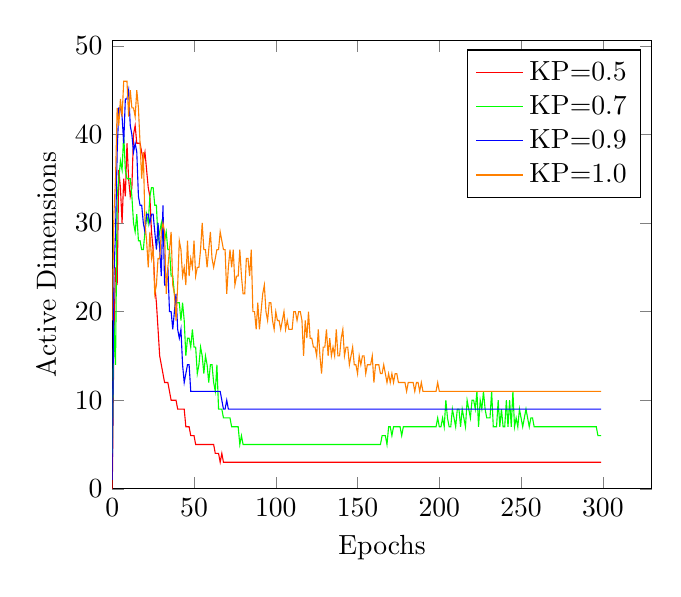
\begin{tikzpicture}\begin{axis}    [% title={Comparison of Dropout Values for Activity},
    xlabel={Epochs},ylabel={Active Dimensions},    xmin=0, xmax=330.0,ymin=0, ymax=50.6,]    \addplot[color=red,]    coordinates {(0,0.0)(1,17.0)(2,25.0)(3,23.0)(4,36.0)(5,34.0)(6,30.0)(7,35.0)(8,33.0)(9,39.0)(10,35.0)(11,33.0)(12,34.0)(13,40.0)(14,41.0)(15,39.0)(16,39.0)(17,39.0)(18,38.0)(19,37.0)(20,38.0)(21,36.0)(22,34.0)(23,33.0)(24,29.0)(25,27.0)(26,23.0)(27,21.0)(28,18.0)(29,15.0)(30,14.0)(31,13.0)(32,12.0)(33,12.0)(34,12.0)(35,11.0)(36,10.0)(37,10.0)(38,10.0)(39,10.0)(40,9.0)(41,9.0)(42,9.0)(43,9.0)(44,9.0)(45,7.0)(46,7.0)(47,7.0)(48,6.0)(49,6.0)(50,6.0)(51,5.0)(52,5.0)(53,5.0)(54,5.0)(55,5.0)(56,5.0)(57,5.0)(58,5.0)(59,5.0)(60,5.0)(61,5.0)(62,5.0)(63,4.0)(64,4.0)(65,4.0)(66,3.0)(67,4.0)(68,3.0)(69,3.0)(70,3.0)(71,3.0)(72,3.0)(73,3.0)(74,3.0)(75,3.0)(76,3.0)(77,3.0)(78,3.0)(79,3.0)(80,3.0)(81,3.0)(82,3.0)(83,3.0)(84,3.0)(85,3.0)(86,3.0)(87,3.0)(88,3.0)(89,3.0)(90,3.0)(91,3.0)(92,3.0)(93,3.0)(94,3.0)(95,3.0)(96,3.0)(97,3.0)(98,3.0)(99,3.0)(100,3.0)(101,3.0)(102,3.0)(103,3.0)(104,3.0)(105,3.0)(106,3.0)(107,3.0)(108,3.0)(109,3.0)(110,3.0)(111,3.0)(112,3.0)(113,3.0)(114,3.0)(115,3.0)(116,3.0)(117,3.0)(118,3.0)(119,3.0)(120,3.0)(121,3.0)(122,3.0)(123,3.0)(124,3.0)(125,3.0)(126,3.0)(127,3.0)(128,3.0)(129,3.0)(130,3.0)(131,3.0)(132,3.0)(133,3.0)(134,3.0)(135,3.0)(136,3.0)(137,3.0)(138,3.0)(139,3.0)(140,3.0)(141,3.0)(142,3.0)(143,3.0)(144,3.0)(145,3.0)(146,3.0)(147,3.0)(148,3.0)(149,3.0)(150,3.0)(151,3.0)(152,3.0)(153,3.0)(154,3.0)(155,3.0)(156,3.0)(157,3.0)(158,3.0)(159,3.0)(160,3.0)(161,3.0)(162,3.0)(163,3.0)(164,3.0)(165,3.0)(166,3.0)(167,3.0)(168,3.0)(169,3.0)(170,3.0)(171,3.0)(172,3.0)(173,3.0)(174,3.0)(175,3.0)(176,3.0)(177,3.0)(178,3.0)(179,3.0)(180,3.0)(181,3.0)(182,3.0)(183,3.0)(184,3.0)(185,3.0)(186,3.0)(187,3.0)(188,3.0)(189,3.0)(190,3.0)(191,3.0)(192,3.0)(193,3.0)(194,3.0)(195,3.0)(196,3.0)(197,3.0)(198,3.0)(199,3.0)(200,3.0)(201,3.0)(202,3.0)(203,3.0)(204,3.0)(205,3.0)(206,3.0)(207,3.0)(208,3.0)(209,3.0)(210,3.0)(211,3.0)(212,3.0)(213,3.0)(214,3.0)(215,3.0)(216,3.0)(217,3.0)(218,3.0)(219,3.0)(220,3.0)(221,3.0)(222,3.0)(223,3.0)(224,3.0)(225,3.0)(226,3.0)(227,3.0)(228,3.0)(229,3.0)(230,3.0)(231,3.0)(232,3.0)(233,3.0)(234,3.0)(235,3.0)(236,3.0)(237,3.0)(238,3.0)(239,3.0)(240,3.0)(241,3.0)(242,3.0)(243,3.0)(244,3.0)(245,3.0)(246,3.0)(247,3.0)(248,3.0)(249,3.0)(250,3.0)(251,3.0)(252,3.0)(253,3.0)(254,3.0)(255,3.0)(256,3.0)(257,3.0)(258,3.0)(259,3.0)(260,3.0)(261,3.0)(262,3.0)(263,3.0)(264,3.0)(265,3.0)(266,3.0)(267,3.0)(268,3.0)(269,3.0)(270,3.0)(271,3.0)(272,3.0)(273,3.0)(274,3.0)(275,3.0)(276,3.0)(277,3.0)(278,3.0)(279,3.0)(280,3.0)(281,3.0)(282,3.0)(283,3.0)(284,3.0)(285,3.0)(286,3.0)(287,3.0)(288,3.0)(289,3.0)(290,3.0)(291,3.0)(292,3.0)(293,3.0)(294,3.0)(295,3.0)(296,3.0)(297,3.0)(298,3.0)(299,3.0)    };    \addplot[color=green,]    coordinates {(0,4.0)(1,19.0)(2,14.0)(3,33.0)(4,35.0)(5,37.0)(6,36.0)(7,40.0)(8,36.0)(9,35.0)(10,35.0)(11,35.0)(12,33.0)(13,30.0)(14,29.0)(15,31.0)(16,28.0)(17,28.0)(18,27.0)(19,27.0)(20,29.0)(21,31.0)(22,30.0)(23,33.0)(24,34.0)(25,34.0)(26,32.0)(27,32.0)(28,28.0)(29,29.0)(30,30.0)(31,28.0)(32,28.0)(33,29.0)(34,27.0)(35,27.0)(36,24.0)(37,24.0)(38,22.0)(39,21.0)(40,21.0)(41,21.0)(42,19.0)(43,21.0)(44,19.0)(45,15.0)(46,17.0)(47,17.0)(48,16.0)(49,18.0)(50,16.0)(51,16.0)(52,13.0)(53,14.0)(54,16.0)(55,15.0)(56,13.0)(57,15.0)(58,14.0)(59,12.0)(60,14.0)(61,14.0)(62,12.0)(63,11.0)(64,14.0)(65,9.0)(66,9.0)(67,9.0)(68,8.0)(69,8.0)(70,8.0)(71,8.0)(72,8.0)(73,7.0)(74,7.0)(75,7.0)(76,7.0)(77,7.0)(78,5.0)(79,6.0)(80,5.0)(81,5.0)(82,5.0)(83,5.0)(84,5.0)(85,5.0)(86,5.0)(87,5.0)(88,5.0)(89,5.0)(90,5.0)(91,5.0)(92,5.0)(93,5.0)(94,5.0)(95,5.0)(96,5.0)(97,5.0)(98,5.0)(99,5.0)(100,5.0)(101,5.0)(102,5.0)(103,5.0)(104,5.0)(105,5.0)(106,5.0)(107,5.0)(108,5.0)(109,5.0)(110,5.0)(111,5.0)(112,5.0)(113,5.0)(114,5.0)(115,5.0)(116,5.0)(117,5.0)(118,5.0)(119,5.0)(120,5.0)(121,5.0)(122,5.0)(123,5.0)(124,5.0)(125,5.0)(126,5.0)(127,5.0)(128,5.0)(129,5.0)(130,5.0)(131,5.0)(132,5.0)(133,5.0)(134,5.0)(135,5.0)(136,5.0)(137,5.0)(138,5.0)(139,5.0)(140,5.0)(141,5.0)(142,5.0)(143,5.0)(144,5.0)(145,5.0)(146,5.0)(147,5.0)(148,5.0)(149,5.0)(150,5.0)(151,5.0)(152,5.0)(153,5.0)(154,5.0)(155,5.0)(156,5.0)(157,5.0)(158,5.0)(159,5.0)(160,5.0)(161,5.0)(162,5.0)(163,5.0)(164,5.0)(165,6.0)(166,6.0)(167,6.0)(168,5.0)(169,7.0)(170,7.0)(171,6.0)(172,7.0)(173,7.0)(174,7.0)(175,7.0)(176,7.0)(177,6.0)(178,7.0)(179,7.0)(180,7.0)(181,7.0)(182,7.0)(183,7.0)(184,7.0)(185,7.0)(186,7.0)(187,7.0)(188,7.0)(189,7.0)(190,7.0)(191,7.0)(192,7.0)(193,7.0)(194,7.0)(195,7.0)(196,7.0)(197,7.0)(198,7.0)(199,8.0)(200,7.0)(201,7.0)(202,8.0)(203,7.0)(204,10.0)(205,8.0)(206,7.0)(207,7.0)(208,9.0)(209,8.0)(210,7.0)(211,9.0)(212,9.0)(213,7.0)(214,9.0)(215,8.0)(216,7.0)(217,10.0)(218,9.0)(219,8.0)(220,10.0)(221,10.0)(222,9.0)(223,11.0)(224,7.0)(225,10.0)(226,9.0)(227,11.0)(228,9.0)(229,8.0)(230,8.0)(231,8.0)(232,11.0)(233,7.0)(234,7.0)(235,7.0)(236,10.0)(237,7.0)(238,9.0)(239,7.0)(240,7.0)(241,10.0)(242,7.0)(243,10.0)(244,7.0)(245,11.0)(246,7.0)(247,8.0)(248,7.0)(249,9.0)(250,8.0)(251,7.0)(252,8.0)(253,9.0)(254,8.0)(255,7.0)(256,8.0)(257,8.0)(258,7.0)(259,7.0)(260,7.0)(261,7.0)(262,7.0)(263,7.0)(264,7.0)(265,7.0)(266,7.0)(267,7.0)(268,7.0)(269,7.0)(270,7.0)(271,7.0)(272,7.0)(273,7.0)(274,7.0)(275,7.0)(276,7.0)(277,7.0)(278,7.0)(279,7.0)(280,7.0)(281,7.0)(282,7.0)(283,7.0)(284,7.0)(285,7.0)(286,7.0)(287,7.0)(288,7.0)(289,7.0)(290,7.0)(291,7.0)(292,7.0)(293,7.0)(294,7.0)(295,7.0)(296,7.0)(297,6.0)(298,6.0)(299,6.0)    };    \addplot[color=blue,]    coordinates {(0,1.0)(1,24.0)(2,29.0)(3,38.0)(4,43.0)(5,43.0)(6,42.0)(7,39.0)(8,44.0)(9,44.0)(10,45.0)(11,41.0)(12,40.0)(13,38.0)(14,39.0)(15,38.0)(16,33.0)(17,32.0)(18,32.0)(19,30.0)(20,29.0)(21,31.0)(22,31.0)(23,30.0)(24,31.0)(25,31.0)(26,29.0)(27,27.0)(28,30.0)(29,27.0)(30,24.0)(31,32.0)(32,23.0)(33,23.0)(34,25.0)(35,20.0)(36,20.0)(37,18.0)(38,20.0)(39,22.0)(40,18.0)(41,17.0)(42,18.0)(43,14.0)(44,12.0)(45,13.0)(46,14.0)(47,14.0)(48,11.0)(49,11.0)(50,11.0)(51,11.0)(52,11.0)(53,11.0)(54,11.0)(55,11.0)(56,11.0)(57,11.0)(58,11.0)(59,11.0)(60,11.0)(61,11.0)(62,11.0)(63,11.0)(64,11.0)(65,11.0)(66,11.0)(67,10.0)(68,9.0)(69,9.0)(70,10.0)(71,9.0)(72,9.0)(73,9.0)(74,9.0)(75,9.0)(76,9.0)(77,9.0)(78,9.0)(79,9.0)(80,9.0)(81,9.0)(82,9.0)(83,9.0)(84,9.0)(85,9.0)(86,9.0)(87,9.0)(88,9.0)(89,9.0)(90,9.0)(91,9.0)(92,9.0)(93,9.0)(94,9.0)(95,9.0)(96,9.0)(97,9.0)(98,9.0)(99,9.0)(100,9.0)(101,9.0)(102,9.0)(103,9.0)(104,9.0)(105,9.0)(106,9.0)(107,9.0)(108,9.0)(109,9.0)(110,9.0)(111,9.0)(112,9.0)(113,9.0)(114,9.0)(115,9.0)(116,9.0)(117,9.0)(118,9.0)(119,9.0)(120,9.0)(121,9.0)(122,9.0)(123,9.0)(124,9.0)(125,9.0)(126,9.0)(127,9.0)(128,9.0)(129,9.0)(130,9.0)(131,9.0)(132,9.0)(133,9.0)(134,9.0)(135,9.0)(136,9.0)(137,9.0)(138,9.0)(139,9.0)(140,9.0)(141,9.0)(142,9.0)(143,9.0)(144,9.0)(145,9.0)(146,9.0)(147,9.0)(148,9.0)(149,9.0)(150,9.0)(151,9.0)(152,9.0)(153,9.0)(154,9.0)(155,9.0)(156,9.0)(157,9.0)(158,9.0)(159,9.0)(160,9.0)(161,9.0)(162,9.0)(163,9.0)(164,9.0)(165,9.0)(166,9.0)(167,9.0)(168,9.0)(169,9.0)(170,9.0)(171,9.0)(172,9.0)(173,9.0)(174,9.0)(175,9.0)(176,9.0)(177,9.0)(178,9.0)(179,9.0)(180,9.0)(181,9.0)(182,9.0)(183,9.0)(184,9.0)(185,9.0)(186,9.0)(187,9.0)(188,9.0)(189,9.0)(190,9.0)(191,9.0)(192,9.0)(193,9.0)(194,9.0)(195,9.0)(196,9.0)(197,9.0)(198,9.0)(199,9.0)(200,9.0)(201,9.0)(202,9.0)(203,9.0)(204,9.0)(205,9.0)(206,9.0)(207,9.0)(208,9.0)(209,9.0)(210,9.0)(211,9.0)(212,9.0)(213,9.0)(214,9.0)(215,9.0)(216,9.0)(217,9.0)(218,9.0)(219,9.0)(220,9.0)(221,9.0)(222,9.0)(223,9.0)(224,9.0)(225,9.0)(226,9.0)(227,9.0)(228,9.0)(229,9.0)(230,9.0)(231,9.0)(232,9.0)(233,9.0)(234,9.0)(235,9.0)(236,9.0)(237,9.0)(238,9.0)(239,9.0)(240,9.0)(241,9.0)(242,9.0)(243,9.0)(244,9.0)(245,9.0)(246,9.0)(247,9.0)(248,9.0)(249,9.0)(250,9.0)(251,9.0)(252,9.0)(253,9.0)(254,9.0)(255,9.0)(256,9.0)(257,9.0)(258,9.0)(259,9.0)(260,9.0)(261,9.0)(262,9.0)(263,9.0)(264,9.0)(265,9.0)(266,9.0)(267,9.0)(268,9.0)(269,9.0)(270,9.0)(271,9.0)(272,9.0)(273,9.0)(274,9.0)(275,9.0)(276,9.0)(277,9.0)(278,9.0)(279,9.0)(280,9.0)(281,9.0)(282,9.0)(283,9.0)(284,9.0)(285,9.0)(286,9.0)(287,9.0)(288,9.0)(289,9.0)(290,9.0)(291,9.0)(292,9.0)(293,9.0)(294,9.0)(295,9.0)(296,9.0)(297,9.0)(298,9.0)(299,9.0)    };    \addplot[color=orange,]    coordinates {(0,19.0)(1,31.0)(2,35.0)(3,43.0)(4,41.0)(5,44.0)(6,42.0)(7,46.0)(8,46.0)(9,46.0)(10,42.0)(11,45.0)(12,43.0)(13,43.0)(14,42.0)(15,45.0)(16,43.0)(17,39.0)(18,35.0)(19,38.0)(20,30.0)(21,28.0)(22,25.0)(23,29.0)(24,26.0)(25,27.0)(26,22.0)(27,23.0)(28,26.0)(29,26.0)(30,29.0)(31,30.0)(32,29.0)(33,22.0)(34,25.0)(35,27.0)(36,29.0)(37,23.0)(38,22.0)(39,19.0)(40,23.0)(41,28.0)(42,27.0)(43,24.0)(44,25.0)(45,23.0)(46,28.0)(47,24.0)(48,26.0)(49,25.0)(50,28.0)(51,24.0)(52,25.0)(53,25.0)(54,27.0)(55,30.0)(56,27.0)(57,27.0)(58,25.0)(59,27.0)(60,29.0)(61,26.0)(62,25.0)(63,26.0)(64,27.0)(65,27.0)(66,29.0)(67,28.0)(68,27.0)(69,27.0)(70,22.0)(71,25.0)(72,27.0)(73,25.0)(74,27.0)(75,23.0)(76,24.0)(77,24.0)(78,27.0)(79,24.0)(80,22.0)(81,22.0)(82,26.0)(83,26.0)(84,24.0)(85,27.0)(86,20.0)(87,20.0)(88,18.0)(89,21.0)(90,18.0)(91,20.0)(92,22.0)(93,23.0)(94,20.0)(95,19.0)(96,21.0)(97,21.0)(98,19.0)(99,18.0)(100,20.0)(101,19.0)(102,19.0)(103,18.0)(104,19.0)(105,20.0)(106,18.0)(107,19.0)(108,18.0)(109,18.0)(110,18.0)(111,20.0)(112,20.0)(113,19.0)(114,20.0)(115,20.0)(116,19.0)(117,15.0)(118,19.0)(119,17.0)(120,20.0)(121,17.0)(122,17.0)(123,16.0)(124,16.0)(125,15.0)(126,18.0)(127,15.0)(128,13.0)(129,16.0)(130,16.0)(131,18.0)(132,15.0)(133,17.0)(134,15.0)(135,16.0)(136,15.0)(137,18.0)(138,15.0)(139,15.0)(140,17.0)(141,18.0)(142,15.0)(143,16.0)(144,16.0)(145,14.0)(146,15.0)(147,16.0)(148,14.0)(149,14.0)(150,13.0)(151,15.0)(152,14.0)(153,15.0)(154,15.0)(155,13.0)(156,14.0)(157,14.0)(158,14.0)(159,15.0)(160,12.0)(161,14.0)(162,14.0)(163,14.0)(164,13.0)(165,13.0)(166,14.0)(167,13.0)(168,12.0)(169,13.0)(170,12.0)(171,13.0)(172,12.0)(173,13.0)(174,13.0)(175,12.0)(176,12.0)(177,12.0)(178,12.0)(179,12.0)(180,11.0)(181,12.0)(182,12.0)(183,12.0)(184,12.0)(185,11.0)(186,12.0)(187,12.0)(188,11.0)(189,12.0)(190,11.0)(191,11.0)(192,11.0)(193,11.0)(194,11.0)(195,11.0)(196,11.0)(197,11.0)(198,11.0)(199,12.0)(200,11.0)(201,11.0)(202,11.0)(203,11.0)(204,11.0)(205,11.0)(206,11.0)(207,11.0)(208,11.0)(209,11.0)(210,11.0)(211,11.0)(212,11.0)(213,11.0)(214,11.0)(215,11.0)(216,11.0)(217,11.0)(218,11.0)(219,11.0)(220,11.0)(221,11.0)(222,11.0)(223,11.0)(224,11.0)(225,11.0)(226,11.0)(227,11.0)(228,11.0)(229,11.0)(230,11.0)(231,11.0)(232,11.0)(233,11.0)(234,11.0)(235,11.0)(236,11.0)(237,11.0)(238,11.0)(239,11.0)(240,11.0)(241,11.0)(242,11.0)(243,11.0)(244,11.0)(245,11.0)(246,11.0)(247,11.0)(248,11.0)(249,11.0)(250,11.0)(251,11.0)(252,11.0)(253,11.0)(254,11.0)(255,11.0)(256,11.0)(257,11.0)(258,11.0)(259,11.0)(260,11.0)(261,11.0)(262,11.0)(263,11.0)(264,11.0)(265,11.0)(266,11.0)(267,11.0)(268,11.0)(269,11.0)(270,11.0)(271,11.0)(272,11.0)(273,11.0)(274,11.0)(275,11.0)(276,11.0)(277,11.0)(278,11.0)(279,11.0)(280,11.0)(281,11.0)(282,11.0)(283,11.0)(284,11.0)(285,11.0)(286,11.0)(287,11.0)(288,11.0)(289,11.0)(290,11.0)(291,11.0)(292,11.0)(293,11.0)(294,11.0)(295,11.0)(296,11.0)(297,11.0)(298,11.0)(299,11.0)    };    \legend{KP=0.5,KP=0.7,KP=0.9,KP=1.0,}\end{axis}\end{tikzpicture}\\
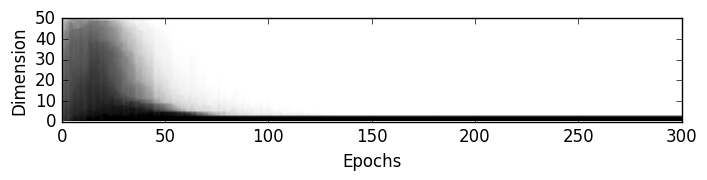
\includegraphics[scale=0.75]{{../img/trial.50.0.5.0.0.1.KP=0.5}.png}\\
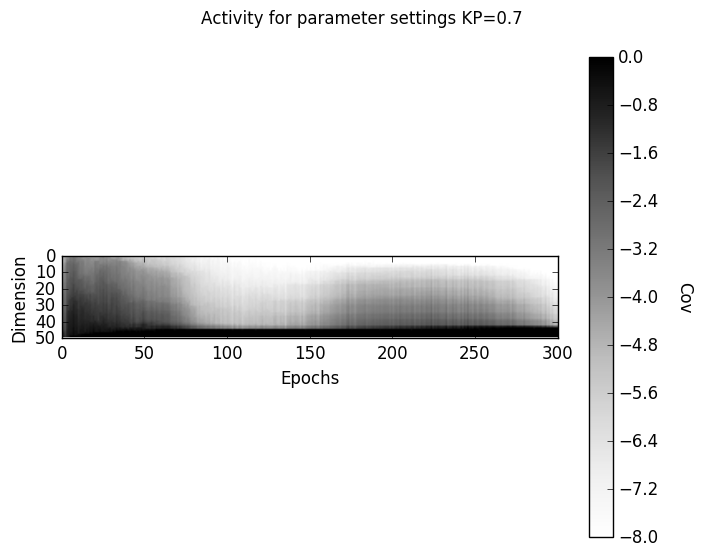
\includegraphics[scale=0.75]{{../img/trial.50.0.7.0.0.1.KP=0.7}.png}\\
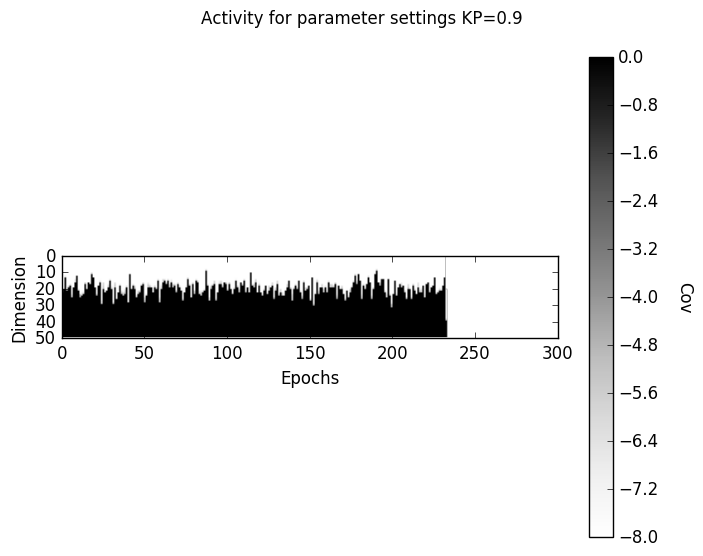
\includegraphics[scale=0.75]{{../img/trial.50.0.9.0.0.1.KP=0.9}.png}\\
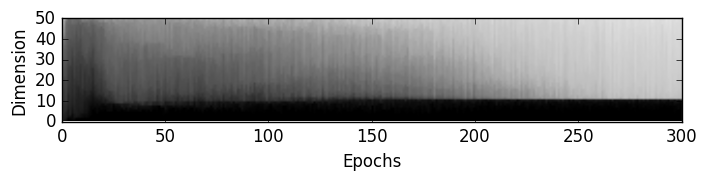
\includegraphics[scale=0.75]{{../img/trial.50.1.0.0.0.1.KP=1.0}.png}\\
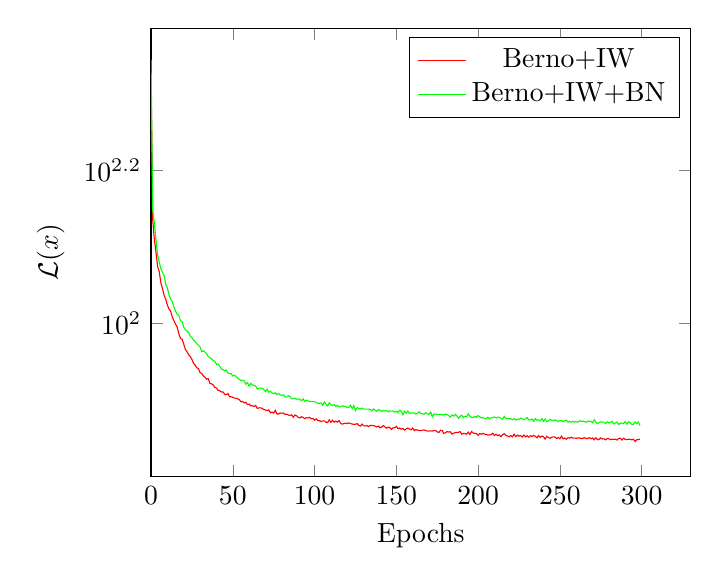
\begin{tikzpicture}\begin{semilogyaxis}    [% title={Comparison of Importance Weighted and Batch Normalized},
    xlabel={Epochs},ylabel={$\mathcal{L}(x)$},    xmin=0.0, xmax=330.0,ymin=63.1280970653, ymax=242.893315674,]    \addplot[color=red,]    coordinates {(0,212.889503881)(1,136.69067473)(2,128.82833134)(3,124.040854936)(4,118.690849804)(5,116.909000924)(6,113.013927626)(7,111.075254586)(8,108.798369917)(9,107.562806091)(10,105.667284851)(11,104.449745872)(12,103.738867798)(13,101.913222407)(14,100.880470165)(15,99.7707582092)(16,98.9113952359)(17,96.9467745001)(18,95.6420740024)(19,95.3488831676)(20,93.9665334251)(21,92.4877756431)(22,91.8431637018)(23,91.0363048068)(24,90.5232136397)(25,89.7399208069)(26,88.7281854803)(27,88.1798480225)(28,87.5367355208)(29,87.3209809875)(30,86.2576438349)(31,86.0276815102)(32,85.4221434021)(33,85.0303677923)(34,84.5800309337)(35,84.7152453891)(36,83.5131790022)(37,83.4104959453)(38,83.1304513758)(39,82.4841615989)(40,82.3764996546)(41,81.7875932936)(42,81.7060721588)(43,81.3806930681)(44,81.4111268546)(45,80.838586731)(46,80.7406091725)(47,81.017188041)(48,80.2124638228)(49,80.2271451361)(50,80.0896083138)(51,79.8871128637)(52,79.8942684867)(53,79.7550364408)(54,79.538298645)(55,79.0118305414)(56,79.0969413133)(57,78.7534699735)(58,78.9117192979)(59,78.3776827171)(60,78.4891304779)(61,78.0464635398)(62,78.1325949721)(63,77.9003106967)(64,78.1739014712)(65,77.4500395133)(66,77.6281871865)(67,77.6110464131)(68,77.474847426)(69,77.2124328683)(70,77.1030504678)(71,76.9742827121)(72,77.1269824912)(73,76.453514002)(74,76.6268032559)(75,76.3920169484)(76,77.0279490245)(77,76.1911592518)(78,76.1912690319)(79,76.4120253546)(80,76.3616653512)(81,76.4200014773)(82,76.1013489741)(83,76.1299544941)(84,75.9456712133)(85,75.8474544456)(86,75.9958151453)(87,75.4516047114)(88,75.9606080211)(89,75.7825870514)(90,75.4166851807)(91,75.2730201028)(92,75.5633785178)(93,75.3926641221)(94,75.1231771504)(95,75.3425059509)(96,75.2793357017)(97,75.42107236)(98,75.0752778209)(99,75.1563735268)(100,74.7741940308)(101,75.0860549094)(102,74.687021852)(103,74.6451232633)(104,74.4814327032)(105,74.6204650948)(106,74.6206243688)(107,74.3239216544)(108,74.2764617642)(109,74.8516898277)(110,74.3182112052)(111,74.7670684121)(112,74.3290488018)(113,74.5695130088)(114,74.3323224362)(115,74.6895237246)(116,74.0510518993)(117,73.9067425815)(118,74.0074700442)(119,74.1338988495)(120,74.0175181926)(121,74.1761847895)(122,74.0235229562)(123,73.9181140345)(124,73.8457655473)(125,73.8702288749)(126,74.0162856362)(127,73.6437659316)(128,73.4565949943)(129,73.9170945116)(130,73.5467081313)(131,73.4937463864)(132,73.5905630146)(133,73.353295621)(134,73.6264864766)(135,73.5908654092)(136,73.5732003923)(137,73.4532649994)(138,73.2716727794)(139,73.465524188)(140,73.112097598)(141,73.2420930204)(142,73.5635126287)(143,73.3090762398)(144,72.9897125105)(145,73.2172430489)(146,73.1516952931)(147,72.7228497869)(148,73.0782187098)(149,73.1016768508)(150,73.4024589885)(151,72.880766879)(152,73.0312317588)(153,72.7873863844)(154,72.9423721105)(155,72.5628787509)(156,72.8360966284)(157,73.047174426)(158,72.8167339325)(159,72.6396780465)(160,73.0304298262)(161,72.4665298601)(162,72.6912430434)(163,72.5760772358)(164,72.4846100339)(165,72.459022411)(166,72.5838312045)(167,72.6003749293)(168,72.5145784413)(169,72.3569016474)(170,72.3737294076)(171,72.4213695249)(172,72.3710491943)(173,72.4755430534)(174,72.4657969249)(175,72.2095316592)(176,72.0375349288)(177,72.5440174311)(178,72.5334384502)(179,71.8655854936)(180,72.008425508)(181,72.254446425)(182,72.1637018724)(183,72.2237791096)(184,71.714810257)(185,71.9142984702)(186,72.0176052856)(187,72.0815261771)(188,72.0838776606)(189,72.2727386128)(190,71.688610285)(191,71.8585383883)(192,71.8177259757)(193,71.7062380357)(194,72.1454219471)(195,71.6026708776)(196,72.2864398055)(197,71.9247254597)(198,71.868394928)(199,71.8450078375)(200,71.4535544239)(201,71.8534567261)(202,71.670494683)(203,71.8755769626)(204,71.7016650391)(205,71.6363452565)(206,71.504623205)(207,71.5315711698)(208,71.587473741)(209,71.8978508828)(210,71.4103687564)(211,71.70563883)(212,71.3756308677)(213,71.5474994174)(214,71.1844528337)(215,71.60504733)(216,71.8060398934)(217,71.4310690862)(218,71.3169561282)(219,71.1020025912)(220,71.425415476)(221,71.1148356559)(222,71.7071190435)(223,71.1754220234)(224,71.483830067)(225,71.261985321)(226,71.4267416937)(227,71.0780576116)(228,71.5027765656)(229,71.1248665203)(230,71.3434074541)(231,71.0519401204)(232,71.3568696039)(233,71.2187969555)(234,71.4516134782)(235,71.2335008032)(236,70.9221232674)(237,71.3969466123)(238,70.9965213568)(239,71.3100876895)(240,71.1295058164)(241,70.6539552723)(242,71.2394960577)(243,70.9955520907)(244,70.8132880679)(245,71.0490945296)(246,71.1247871052)(247,71.0870736417)(248,70.7841236739)(249,70.9903914504)(250,70.7095126967)(251,71.2655674189)(252,70.6899923706)(253,70.8693695623)(254,70.6116099063)(255,70.951697138)(256,70.8354414368)(257,71.0545902252)(258,70.8714400898)(259,70.8538174022)(260,70.822078039)(261,70.8707302163)(262,70.8950232905)(263,70.7760084395)(264,70.7706362083)(265,70.9704128127)(266,70.7572787822)(267,70.7819294947)(268,70.9383078766)(269,70.7281015916)(270,70.8945835599)(271,70.482622972)(272,70.93528905)(273,70.5277008334)(274,70.5941716211)(275,70.8907409599)(276,70.6606239388)(277,70.7143197632)(278,70.4889673545)(279,70.7734613106)(280,70.716083048)(281,70.5357097002)(282,70.6280721283)(283,70.5701076577)(284,70.6263676938)(285,70.4352469635)(286,70.7839288816)(287,70.8557285656)(288,70.4485128229)(289,70.8420001637)(290,70.5595037981)(291,70.5228122572)(292,70.6055964106)(293,70.5968888716)(294,70.4848312725)(295,70.6190093855)(296,70.1423300726)(297,70.5032779763)(298,70.5609679066)(299,70.6179385029)    };    \addplot[color=green,]    coordinates {(0,220.812105158)(1,140.868051827)(2,135.319417752)(3,128.724276525)(4,122.955164934)(5,120.300830952)(6,117.842742795)(7,116.64050999)(8,115.456067366)(9,112.34451896)(10,111.265299988)(11,108.952617645)(12,107.563851083)(13,106.774169367)(14,105.103744632)(15,103.802531835)(16,102.803668574)(17,102.481998249)(18,100.802762729)(19,100.585010515)(20,98.9090365462)(21,98.1169030346)(22,97.765475991)(23,97.2764186928)(24,96.245937181)(25,95.8124569841)(26,95.1456111839)(27,94.6529702898)(28,94.1195864868)(29,93.6386244618)(30,93.1986750516)(31,91.8884819724)(32,92.1219651656)(33,91.7660386519)(34,91.250533586)(35,90.5151538641)(36,90.2425081288)(37,89.9071646812)(38,89.4961200783)(39,89.1786010881)(40,88.4559831515)(41,88.51847229)(42,87.9428533242)(43,87.1944852101)(44,87.0648347751)(45,86.7229512579)(46,86.9227582203)(47,86.1712326466)(48,85.950587068)(49,86.04926608)(50,85.3923743786)(51,85.5322129267)(52,85.3271336781)(53,84.8019374084)(54,84.536986951)(55,84.2305892389)(56,84.3286683377)(57,84.1522436732)(58,83.3012238104)(59,83.7155057456)(60,82.7992233693)(61,83.5205334057)(62,83.1124755651)(63,83.0196700356)(64,82.8275105979)(65,82.1291870949)(66,82.3226089686)(67,82.3403921648)(68,82.3120443171)(69,81.9174896448)(70,81.5030302568)(71,82.0591559809)(72,81.3132039018)(73,81.591406354)(74,81.1437691914)(75,80.9562143222)(76,81.1953004109)(77,80.6989246923)(78,81.0439923997)(79,80.7104799097)(80,80.579273647)(81,80.6894023687)(82,80.1604832944)(83,80.1868576397)(84,80.4712490706)(85,80.2842603579)(86,79.7442494479)(87,79.7343605735)(88,79.9086901647)(89,79.635063428)(90,79.741575685)(91,79.5902122983)(92,79.2991520483)(93,79.7187010609)(94,79.1092982483)(95,79.4226407693)(96,79.2733724282)(97,79.1051692338)(98,79.0754059809)(99,79.1018828097)(100,79.0593816376)(101,78.9150700933)(102,78.6440699699)(103,78.6818985402)(104,78.7929203033)(105,78.1865223347)(106,79.0145359802)(107,78.4409182462)(108,78.0524690108)(109,78.8077469358)(110,78.2960041046)(111,78.1936078644)(112,78.3528583457)(113,77.9041483238)(114,78.1752235205)(115,77.8163253368)(116,77.9147369385)(117,78.0464619376)(118,77.9532819644)(119,77.9274888819)(120,77.6990697479)(121,77.7212414135)(122,78.2119804313)(123,77.451852091)(124,78.1315626803)(125,76.9649418432)(126,77.6510731576)(127,77.4836851571)(128,77.3073894709)(129,77.5475659943)(130,77.2900101055)(131,77.294678206)(132,77.3047630587)(133,77.2909118236)(134,77.2878407634)(135,76.902970907)(136,77.3512902208)(137,77.1018692849)(138,76.7875662162)(139,77.2080883581)(140,77.0465301098)(141,76.7734781647)(142,76.9981128554)(143,76.8602037048)(144,77.0179359089)(145,76.6783211795)(146,76.887396268)(147,76.8487717438)(148,76.8828933646)(149,76.647767112)(150,76.8185476893)(151,76.4525053753)(152,77.0563210227)(153,76.8780969932)(154,75.9855017992)(155,76.8270853493)(156,76.3929172169)(157,76.8689556191)(158,76.309076219)(159,76.3741976166)(160,76.4659639948)(161,76.4167646165)(162,76.1588406788)(163,76.3985902058)(164,76.6891410065)(165,76.2885811199)(166,76.2813544395)(167,76.1354372267)(168,76.4683616222)(169,76.2195049425)(170,76.0912478707)(171,76.6379284737)(172,75.5368430675)(173,76.2009703549)(174,76.1571691686)(175,76.094223286)(176,76.0969603105)(177,76.0537287279)(178,76.031106505)(179,75.9697008722)(180,76.1766836964)(181,76.0215624861)(182,75.862494486)(183,75.431596867)(184,75.9766488231)(185,75.7119712067)(186,76.0821262498)(187,75.7707103799)(188,75.1897688363)(189,75.6704169533)(190,75.9127686449)(191,75.4278393763)(192,75.6543837253)(193,75.6135286505)(194,76.2010392206)(195,75.6841124101)(196,75.3987940424)(197,75.3748238234)(198,75.6606351887)(199,75.4237091203)(200,75.814623961)(201,75.5699364263)(202,75.2985267292)(203,75.3570597284)(204,75.1684181213)(205,75.1631805767)(206,75.4559900457)(207,75.1224482172)(208,75.3214972063)(209,75.3767447038)(210,75.5251281738)(211,75.2924619501)(212,75.4850157166)(213,75.4524022883)(214,75.191533869)(215,75.0114420249)(216,75.6158445601)(217,75.0702012426)(218,75.0961439167)(219,75.124752121)(220,75.1005330519)(221,74.893462566)(222,75.1368557531)(223,74.8167615856)(224,74.9818515986)(225,74.9404246035)(226,75.2453195329)(227,75.1283115734)(228,74.9109797738)(229,75.103415777)(230,75.3592353058)(231,74.8492726482)(232,74.8929144565)(233,75.032299118)(234,74.5508918693)(235,75.1469980205)(236,74.8126035794)(237,74.8305967782)(238,74.6399993966)(239,75.1417248535)(240,74.556847874)(241,75.0714584628)(242,74.4212250103)(243,74.6612699266)(244,74.9332658733)(245,74.7995458221)(246,74.6834466622)(247,74.8652081229)(248,74.724238524)(249,74.4261099451)(250,74.7198648904)(251,74.7438465743)(252,74.4551574222)(253,74.6536740459)(254,74.7526102794)(255,74.3327881414)(256,74.5383223516)(257,74.3206366036)(258,74.522478603)(259,74.3381154216)(260,74.4665795552)(261,74.3358595623)(262,74.6770175864)(263,74.5301153842)(264,74.5491240345)(265,74.5142330655)(266,74.2829835094)(267,74.5868861389)(268,74.5018216705)(269,74.5457204853)(270,74.2275134763)(271,74.8797874797)(272,74.3535444294)(273,73.9741289312)(274,74.2580836209)(275,74.3988033711)(276,74.3752106198)(277,74.3335512335)(278,74.0707263738)(279,74.4006223158)(280,74.1427292494)(281,74.3383737044)(282,74.5402551686)(283,73.9278499881)(284,74.1787790402)(285,74.3597446858)(286,73.8246305778)(287,74.1425923504)(288,74.0815582622)(289,74.0791946827)(290,74.4631946841)(291,73.9177805467)(292,74.4376518111)(293,74.2326508817)(294,73.8226823009)(295,73.8183200836)(296,74.3854140889)(297,74.0012052363)(298,74.3635426539)(299,73.5976050429)    };    \legend{Berno+IW,Berno+IW+BN,}\end{semilogyaxis}\end{tikzpicture}\\
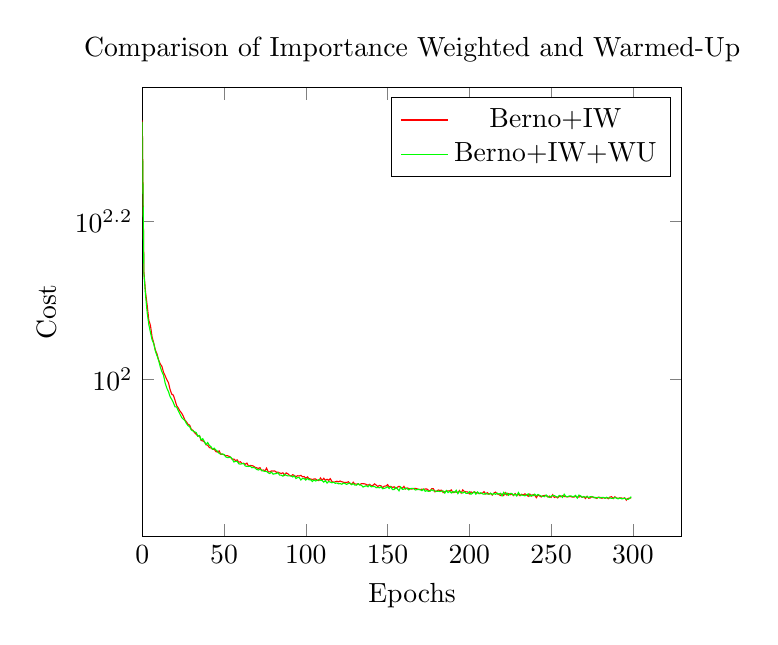
\begin{tikzpicture}\begin{semilogyaxis}    [title={Comparison of Importance Weighted and Warmed-Up},    xlabel={Epochs},ylabel={Cost},    xmin=0.0, xmax=330.0,ymin=63.1280970653, ymax=234.178454269,]    \addplot[color=red,]    coordinates {(0,212.889503881)(1,136.69067473)(2,128.82833134)(3,124.040854936)(4,118.690849804)(5,116.909000924)(6,113.013927626)(7,111.075254586)(8,108.798369917)(9,107.562806091)(10,105.667284851)(11,104.449745872)(12,103.738867798)(13,101.913222407)(14,100.880470165)(15,99.7707582092)(16,98.9113952359)(17,96.9467745001)(18,95.6420740024)(19,95.3488831676)(20,93.9665334251)(21,92.4877756431)(22,91.8431637018)(23,91.0363048068)(24,90.5232136397)(25,89.7399208069)(26,88.7281854803)(27,88.1798480225)(28,87.5367355208)(29,87.3209809875)(30,86.2576438349)(31,86.0276815102)(32,85.4221434021)(33,85.0303677923)(34,84.5800309337)(35,84.7152453891)(36,83.5131790022)(37,83.4104959453)(38,83.1304513758)(39,82.4841615989)(40,82.3764996546)(41,81.7875932936)(42,81.7060721588)(43,81.3806930681)(44,81.4111268546)(45,80.838586731)(46,80.7406091725)(47,81.017188041)(48,80.2124638228)(49,80.2271451361)(50,80.0896083138)(51,79.8871128637)(52,79.8942684867)(53,79.7550364408)(54,79.538298645)(55,79.0118305414)(56,79.0969413133)(57,78.7534699735)(58,78.9117192979)(59,78.3776827171)(60,78.4891304779)(61,78.0464635398)(62,78.1325949721)(63,77.9003106967)(64,78.1739014712)(65,77.4500395133)(66,77.6281871865)(67,77.6110464131)(68,77.474847426)(69,77.2124328683)(70,77.1030504678)(71,76.9742827121)(72,77.1269824912)(73,76.453514002)(74,76.6268032559)(75,76.3920169484)(76,77.0279490245)(77,76.1911592518)(78,76.1912690319)(79,76.4120253546)(80,76.3616653512)(81,76.4200014773)(82,76.1013489741)(83,76.1299544941)(84,75.9456712133)(85,75.8474544456)(86,75.9958151453)(87,75.4516047114)(88,75.9606080211)(89,75.7825870514)(90,75.4166851807)(91,75.2730201028)(92,75.5633785178)(93,75.3926641221)(94,75.1231771504)(95,75.3425059509)(96,75.2793357017)(97,75.42107236)(98,75.0752778209)(99,75.1563735268)(100,74.7741940308)(101,75.0860549094)(102,74.687021852)(103,74.6451232633)(104,74.4814327032)(105,74.6204650948)(106,74.6206243688)(107,74.3239216544)(108,74.2764617642)(109,74.8516898277)(110,74.3182112052)(111,74.7670684121)(112,74.3290488018)(113,74.5695130088)(114,74.3323224362)(115,74.6895237246)(116,74.0510518993)(117,73.9067425815)(118,74.0074700442)(119,74.1338988495)(120,74.0175181926)(121,74.1761847895)(122,74.0235229562)(123,73.9181140345)(124,73.8457655473)(125,73.8702288749)(126,74.0162856362)(127,73.6437659316)(128,73.4565949943)(129,73.9170945116)(130,73.5467081313)(131,73.4937463864)(132,73.5905630146)(133,73.353295621)(134,73.6264864766)(135,73.5908654092)(136,73.5732003923)(137,73.4532649994)(138,73.2716727794)(139,73.465524188)(140,73.112097598)(141,73.2420930204)(142,73.5635126287)(143,73.3090762398)(144,72.9897125105)(145,73.2172430489)(146,73.1516952931)(147,72.7228497869)(148,73.0782187098)(149,73.1016768508)(150,73.4024589885)(151,72.880766879)(152,73.0312317588)(153,72.7873863844)(154,72.9423721105)(155,72.5628787509)(156,72.8360966284)(157,73.047174426)(158,72.8167339325)(159,72.6396780465)(160,73.0304298262)(161,72.4665298601)(162,72.6912430434)(163,72.5760772358)(164,72.4846100339)(165,72.459022411)(166,72.5838312045)(167,72.6003749293)(168,72.5145784413)(169,72.3569016474)(170,72.3737294076)(171,72.4213695249)(172,72.3710491943)(173,72.4755430534)(174,72.4657969249)(175,72.2095316592)(176,72.0375349288)(177,72.5440174311)(178,72.5334384502)(179,71.8655854936)(180,72.008425508)(181,72.254446425)(182,72.1637018724)(183,72.2237791096)(184,71.714810257)(185,71.9142984702)(186,72.0176052856)(187,72.0815261771)(188,72.0838776606)(189,72.2727386128)(190,71.688610285)(191,71.8585383883)(192,71.8177259757)(193,71.7062380357)(194,72.1454219471)(195,71.6026708776)(196,72.2864398055)(197,71.9247254597)(198,71.868394928)(199,71.8450078375)(200,71.4535544239)(201,71.8534567261)(202,71.670494683)(203,71.8755769626)(204,71.7016650391)(205,71.6363452565)(206,71.504623205)(207,71.5315711698)(208,71.587473741)(209,71.8978508828)(210,71.4103687564)(211,71.70563883)(212,71.3756308677)(213,71.5474994174)(214,71.1844528337)(215,71.60504733)(216,71.8060398934)(217,71.4310690862)(218,71.3169561282)(219,71.1020025912)(220,71.425415476)(221,71.1148356559)(222,71.7071190435)(223,71.1754220234)(224,71.483830067)(225,71.261985321)(226,71.4267416937)(227,71.0780576116)(228,71.5027765656)(229,71.1248665203)(230,71.3434074541)(231,71.0519401204)(232,71.3568696039)(233,71.2187969555)(234,71.4516134782)(235,71.2335008032)(236,70.9221232674)(237,71.3969466123)(238,70.9965213568)(239,71.3100876895)(240,71.1295058164)(241,70.6539552723)(242,71.2394960577)(243,70.9955520907)(244,70.8132880679)(245,71.0490945296)(246,71.1247871052)(247,71.0870736417)(248,70.7841236739)(249,70.9903914504)(250,70.7095126967)(251,71.2655674189)(252,70.6899923706)(253,70.8693695623)(254,70.6116099063)(255,70.951697138)(256,70.8354414368)(257,71.0545902252)(258,70.8714400898)(259,70.8538174022)(260,70.822078039)(261,70.8707302163)(262,70.8950232905)(263,70.7760084395)(264,70.7706362083)(265,70.9704128127)(266,70.7572787822)(267,70.7819294947)(268,70.9383078766)(269,70.7281015916)(270,70.8945835599)(271,70.482622972)(272,70.93528905)(273,70.5277008334)(274,70.5941716211)(275,70.8907409599)(276,70.6606239388)(277,70.7143197632)(278,70.4889673545)(279,70.7734613106)(280,70.716083048)(281,70.5357097002)(282,70.6280721283)(283,70.5701076577)(284,70.6263676938)(285,70.4352469635)(286,70.7839288816)(287,70.8557285656)(288,70.4485128229)(289,70.8420001637)(290,70.5595037981)(291,70.5228122572)(292,70.6055964106)(293,70.5968888716)(294,70.4848312725)(295,70.6190093855)(296,70.1423300726)(297,70.5032779763)(298,70.5609679066)(299,70.6179385029)    };    \addplot[color=green,]    coordinates {(0,211.920771235)(1,136.041950406)(2,127.655567821)(3,121.377622819)(4,117.200239147)(5,114.557719255)(6,112.116237765)(7,110.84459438)(8,108.501328)(9,106.994591078)(10,105.528599104)(11,103.523439331)(12,102.1049311)(13,101.044200897)(14,98.7788123946)(15,97.3334535911)(16,96.3747294894)(17,94.9241513478)(18,94.1876848117)(19,93.2820657765)(20,92.1499564431)(21,92.0965787853)(22,91.0992267262)(23,90.258514758)(24,89.367028656)(25,88.9131237516)(26,88.5632063016)(27,87.767957944)(28,87.2004882396)(29,86.9265007296)(30,86.1039954307)(31,85.8721412659)(32,85.6376069225)(33,85.4787972051)(34,84.5375452215)(35,84.7001387995)(36,83.6577368858)(37,83.947080737)(38,83.2251933774)(39,82.5260546667)(40,83.0149431818)(41,82.3260683649)(42,82.0198558253)(43,81.4007761314)(44,81.6464194419)(45,81.2116883087)(46,80.9339801233)(47,80.4093423184)(48,80.2538064506)(49,80.26445626)(50,80.1754982549)(51,79.6065968947)(52,79.4661076424)(53,79.4585576491)(54,79.5529119804)(55,79.1475428841)(56,78.4317886353)(57,78.5672041876)(58,78.5849059296)(59,78.0135896163)(60,77.9302610571)(61,78.0612969971)(62,78.0728800826)(63,77.4989095861)(64,77.4372096252)(65,77.4075387226)(66,77.4833906486)(67,77.1108856895)(68,77.1884387693)(69,77.0652495228)(70,76.731728259)(71,76.6167685491)(72,76.7790292775)(73,76.5561487024)(74,76.3609124687)(75,76.3262932101)(76,76.3038299006)(77,75.9853085813)(78,75.8234346841)(79,76.1432714566)(80,75.6845736278)(81,75.7622598683)(82,75.8358496371)(83,75.9875228327)(84,75.4749721943)(85,75.4622674214)(86,75.2420097698)(87,75.6665474632)(88,75.4173044517)(89,75.3114855055)(90,75.3042652408)(91,75.304190334)(92,75.0652448966)(93,75.300028097)(94,74.7269321858)(95,74.946974633)(96,74.9376493211)(97,74.3935957822)(98,74.7417864921)(99,74.6863958948)(100,74.3666138042)(101,74.7649751837)(102,74.4365995372)(103,74.4630230644)(104,74.0690942868)(105,74.4223918013)(106,74.1677435858)(107,74.364454852)(108,74.4814361225)(109,74.3563543701)(110,74.2843151301)(111,73.9439342429)(112,74.253199671)(113,73.7365618619)(114,74.0730549552)(115,73.9424624426)(116,73.8065217244)(117,73.9410490071)(118,73.6878705528)(119,73.7514558896)(120,73.5626132202)(121,73.6353796248)(122,73.4780480055)(123,73.7383365909)(124,73.6388123183)(125,73.4429614743)(126,73.6361689412)(127,73.7351134422)(128,73.4076615212)(129,73.5874217502)(130,73.2892312969)(131,73.2766345978)(132,73.5973419189)(133,73.3347916274)(134,73.2807842185)(135,72.8754071669)(136,73.0309365359)(137,73.1606336282)(138,72.9356776567)(139,73.3240285353)(140,72.9366025196)(141,72.9952358107)(142,73.0188198159)(143,72.7373005329)(144,72.8023182193)(145,72.7158220118)(146,72.9424673878)(147,72.5235708063)(148,72.6176831956)(149,72.710772067)(150,72.9506710538)(151,72.5792145538)(152,72.9156984433)(153,72.350460968)(154,72.3601283472)(155,72.8084296348)(156,72.5080196381)(157,72.0916944885)(158,72.8939842363)(159,72.4100078236)(160,72.4259916826)(161,72.6570126343)(162,72.5569174957)(163,72.2766546492)(164,72.5522474878)(165,72.6117680151)(166,72.5266255327)(167,72.2553674594)(168,72.3381537975)(169,72.409844291)(170,72.3197260839)(171,72.1210739621)(172,72.4554304712)(173,71.9798968367)(174,72.1140852148)(175,71.9664068465)(176,72.0398827431)(177,72.3290373785)(178,72.0786895613)(179,72.0804263652)(180,71.9566899109)(181,72.0199571228)(182,71.934291909)(183,72.0198452967)(184,72.0492370259)(185,71.6058983959)(186,72.1443767201)(187,71.7032741547)(188,72.0154839186)(189,71.6328542813)(190,71.9075974829)(191,71.724543027)(192,72.2001169101)(193,71.4893339469)(194,71.9989465609)(195,71.7248961431)(196,71.6155355904)(197,71.8625546958)(198,71.5448267087)(199,71.5348938821)(200,71.8927913874)(201,71.3641139291)(202,71.5757099152)(203,71.8791705461)(204,71.3734206529)(205,71.8555987896)(206,71.484037642)(207,71.6702431141)(208,71.4488757324)(209,71.3613694555)(210,71.5625690668)(211,71.4003565147)(212,71.3800912059)(213,71.5839483781)(214,71.2877472617)(215,71.524486944)(216,71.3508754522)(217,71.598925379)(218,71.382131424)(219,71.5678360124)(220,71.0216996072)(221,71.747851396)(222,71.3518445795)(223,71.618864323)(224,71.1494074457)(225,71.5245897744)(226,71.5174071919)(227,71.1610129131)(228,71.3841708721)(229,71.0022963645)(230,71.7317855974)(231,71.1931494349)(232,71.2135812586)(233,71.137647171)(234,71.0353393555)(235,71.2289615215)(236,71.4292991708)(237,70.9530152269)(238,71.2058131478)(239,71.0402913943)(240,71.3815405204)(241,71.0421990273)(242,71.3243312489)(243,71.1418269834)(244,70.98499287)(245,70.9436188715)(246,70.8601362124)(247,71.2015867962)(248,70.8859353013)(249,70.7014370034)(250,70.9372913707)(251,71.1071626767)(252,71.0702215923)(253,70.9006895516)(254,70.7234609569)(255,71.1173128163)(256,71.0182432417)(257,70.705510351)(258,71.3739971924)(259,70.9233442272)(260,70.824895505)(261,70.9906147697)(262,71.0317549272)(263,70.8631683003)(264,70.9017379622)(265,71.1260205356)(266,70.5664304837)(267,71.1922574269)(268,71.0396257782)(269,70.7427878848)(270,70.8481825534)(271,70.7551518041)(272,70.8912699682)(273,70.6720841703)(274,70.8669612746)(275,70.8213413793)(276,70.7864981842)(277,70.5794426311)(278,70.681183867)(279,70.7142483451)(280,70.5600470179)(281,70.7070504691)(282,70.7109043052)(283,70.5212578167)(284,70.7369764571)(285,70.5565758722)(286,70.6001445909)(287,70.5064651142)(288,70.5170895316)(289,70.6795578072)(290,70.5741186662)(291,70.4079902926)(292,70.5973380557)(293,70.4269882133)(294,70.4426253232)(295,70.5469852933)(296,70.359163097)(297,70.2867510431)(298,70.4760524542)(299,70.8463656408)    };    \legend{Berno+IW,Berno+IW+WU,}\end{semilogyaxis}\end{tikzpicture}\\
\begin{tikzpicture}\begin{axis}    [% title={Comparison of Dimension Values for Cost},
    xlabel={Epochs},ylabel={$\mathcal{L}(x)$},    xmin=0, xmax=330.0,ymin=0, ymax=234.178454269,]    \addplot[color=red,]    coordinates {(0,212.64562518)(1,136.790049189)(2,129.450027147)(3,124.806456646)(4,119.629016543)(5,115.866283098)(6,113.65281791)(7,113.216522466)(8,112.390473661)(9,112.459851352)(10,110.561585)(11,110.58909249)(12,110.582688959)(13,108.98578168)(14,108.174572268)(15,106.94951391)(16,106.52779971)(17,105.903768741)(18,106.490196048)(19,104.782711417)(20,104.510796273)(21,104.317927634)(22,104.268410977)(23,104.529566068)(24,103.975174047)(25,103.529354553)(26,104.223509424)(27,103.341782157)(28,103.223864885)(29,103.04055112)(30,102.511857203)(31,102.44037004)(32,102.624933264)(33,102.595905859)(34,102.056924605)(35,102.161272638)(36,102.107101718)(37,102.169749908)(38,101.139953877)(39,100.591849768)(40,101.12034163)(41,101.795387601)(42,100.565506148)(43,100.449325894)(44,100.776369449)(45,99.805602306)(46,100.013280903)(47,99.3922403648)(48,99.8124241222)(49,99.8443745006)(50,98.8423816612)(51,99.0189324119)(52,99.0970941301)(53,98.9608595831)(54,98.8333989091)(55,98.6930469444)(56,98.4971124406)(57,98.5305879628)(58,97.8677001537)(59,97.9693040328)(60,97.4770084312)(61,96.9026780007)(62,97.0764308583)(63,96.6972712846)(64,96.7026261208)(65,96.0112938621)(66,96.3034130166)(67,96.2243750139)(68,96.2673697316)(69,95.4720721852)(70,95.5351370933)(71,96.0084017944)(72,95.6774275901)(73,95.3824603826)(74,95.3175074768)(75,95.4738596552)(76,94.8010714999)(77,95.0208831926)(78,95.1377222651)(79,94.8573893877)(80,94.5328298118)(81,94.9248980435)(82,94.1536433272)(83,94.8404233482)(84,93.9009531888)(85,94.5247418768)(86,94.003690463)(87,94.4343333712)(88,94.3249619779)(89,93.9180274963)(90,93.8450731312)(91,93.9086502769)(92,94.4001156061)(93,94.0345778448)(94,93.4910698076)(95,93.7357471258)(96,93.620851052)(97,93.2118634033)(98,93.4317974992)(99,92.9778021379)(100,93.178931108)(101,93.0553935103)(102,92.6037774519)(103,93.4789959023)(104,92.8939061252)(105,92.0754372198)(106,92.9563021989)(107,92.5446649864)(108,93.3927328352)(109,92.1056706377)(110,92.9950072132)(111,92.6017806591)(112,92.3819902455)(113,92.4697180453)(114,92.4149521568)(115,92.1641739585)(116,92.02042099)(117,92.5232783647)(118,92.1915834462)(119,92.5636461709)(120,91.499622664)(121,92.2548089045)(122,91.5942985951)(123,91.8366348821)(124,92.4226245949)(125,91.5781864513)(126,91.9253713434)(127,91.8256563915)(128,91.6219063776)(129,91.6083890742)(130,91.9204267606)(131,91.7192824485)(132,91.8309332414)(133,91.6001627697)(134,91.7785151256)(135,91.9343934909)(136,90.9708414945)(137,91.8394788014)(138,91.2352882108)(139,91.3972491316)(140,91.053236084)(141,91.6676521024)(142,91.2520715193)(143,90.921548344)(144,91.0097028836)(145,91.2740852633)(146,91.2315159746)(147,91.3598694957)(148,91.3016590465)(149,91.116959173)(150,90.8034104503)(151,90.3776094263)(152,91.37105982)(153,90.459977847)(154,91.4105793762)(155,90.7973893738)(156,90.6487164862)(157,90.7972389776)(158,90.9623546531)(159,90.6492305825)(160,90.7841757202)(161,91.0368552191)(162,90.3820919384)(163,91.0561155978)(164,90.7019770119)(165,90.1748568309)(166,90.2482923057)(167,91.0781902244)(168,90.8552395491)(169,90.2778696095)(170,90.8713644132)(171,90.8574212785)(172,90.5594718933)(173,90.5203334323)(174,90.1041105929)(175,90.9452550437)(176,90.5799438199)(177,90.4445606578)(178,89.8594377136)(179,90.4176010825)(180,89.9413424336)(181,90.0970399891)(182,90.3487412054)(183,90.1685987715)(184,90.0106440666)(185,90.0788917403)(186,90.1420660817)(187,90.2814241583)(188,89.9337448814)(189,89.6335220406)(190,90.2058405998)(191,90.229971154)(192,89.4233127663)(193,89.7349503118)(194,89.8484557689)(195,89.8542760398)(196,90.0848807595)(197,89.4077824055)(198,89.7168458696)(199,90.091522307)(200,89.4497258412)(201,89.6172247592)(202,89.9387405673)(203,89.9406651445)(204,89.3606143882)(205,89.6490585882)(206,89.088557878)(207,89.4311926131)(208,89.4872697171)(209,89.221857064)(210,90.0243047541)(211,89.536120439)(212,89.5942551977)(213,89.4242223566)(214,89.2525826402)(215,89.6891998638)(216,89.0924630599)(217,89.1673583984)(218,88.8423385204)(219,89.1576703436)(220,89.1534130859)(221,89.1359509277)(222,88.7960712086)(223,88.941094187)(224,88.6995326233)(225,89.2326003057)(226,88.8880756031)(227,88.8336592657)(228,88.8789133731)(229,88.9285824793)(230,89.0151744218)(231,88.7847638356)(232,88.2256437544)(233,88.9106356118)(234,88.7218838778)(235,88.8426841042)(236,88.7913392084)(237,88.4047441101)(238,89.1131186745)(239,89.1689117987)(240,88.7673648626)(241,88.5378052035)(242,87.9620528481)(243,88.7573857672)(244,88.4587245456)(245,88.5162724165)(246,88.3751076438)(247,88.0754129999)(248,88.4787031139)(249,88.6045204995)(250,87.8536755232)(251,88.6177316284)(252,88.437724221)(253,88.4052790971)(254,88.2066417209)(255,88.8713390697)(256,87.9724222495)(257,87.8995355086)(258,88.4342787864)(259,88.268974755)(260,87.899311891)(261,87.7624074346)(262,88.4280469721)(263,87.8955852509)(264,88.0528344588)(265,88.1902413247)(266,88.0831458768)(267,88.0866466037)(268,88.1232280939)(269,87.7360985426)(270,87.8346880687)(271,88.1459167758)(272,87.4026767384)(273,87.6557292037)(274,88.5485077598)(275,87.7667722667)(276,87.4979941212)(277,87.977197113)(278,87.5508903642)(279,87.6130116272)(280,87.648626709)(281,87.6456446145)(282,87.3224346924)(283,87.8284001576)(284,87.7360886036)(285,87.74671789)(286,87.6882106365)(287,88.4206697568)(288,87.53956767)(289,87.2739833485)(290,87.8526529)(291,87.535925071)(292,87.5970885329)(293,87.4183481945)(294,87.3325238661)(295,87.8397986811)(296,87.0593926586)(297,87.8364493075)(298,87.3532575989)(299,87.6076428569)    };    \addplot[color=green,]    coordinates {(0,210.501984849)(1,137.075507604)(2,129.281337502)(3,124.670307298)(4,118.349319444)(5,114.545375671)(6,111.9949311)(7,108.483689686)(8,104.742418241)(9,102.436671475)(10,100.699877541)(11,99.6592659551)(12,97.9936723189)(13,97.0524140653)(14,96.2055522572)(15,94.8494610318)(16,93.8501225558)(17,92.5859065801)(18,91.9925247747)(19,91.100423473)(20,90.5070888727)(21,89.7772999573)(22,88.9261402546)(23,88.6802403606)(24,87.8085623446)(25,87.7236609303)(26,87.0449466428)(27,87.0122712985)(28,86.5224651822)(29,85.9470366044)(30,86.0935158053)(31,85.5794501634)(32,85.1979700401)(33,85.1442778709)(34,84.9510265281)(35,84.3852848608)(36,83.976246546)(37,84.2003873582)(38,83.8376353593)(39,83.4123169778)(40,83.4118772541)(41,83.604622123)(42,83.5064559728)(43,83.1131862432)(44,82.5573041673)(45,82.7421252858)(46,82.2595257985)(47,82.2053425321)(48,82.1005601085)(49,82.0737834376)(50,82.106804227)(51,81.9768792308)(52,81.8916197551)(53,81.331090296)(54,81.4447430559)(55,81.3403038788)(56,81.0759906145)(57,81.0545472648)(58,81.2044740434)(59,81.007102675)(60,80.9177202606)(61,80.6498646476)(62,80.734708252)(63,80.7922399556)(64,80.5605086725)(65,80.7934116086)(66,80.665143932)(67,80.3323184135)(68,80.0511437295)(69,80.3284948106)(70,80.0951102794)(71,80.0512655778)(72,79.7207394687)(73,79.6659372989)(74,79.7284209442)(75,79.4676317042)(76,79.7636759047)(77,79.8371999983)(78,79.6556122034)(79,79.5083737391)(80,79.3074531278)(81,79.2636697943)(82,79.2930197421)(83,79.3694778997)(84,79.092231695)(85,79.123703856)(86,79.1527527202)(87,79.1723667561)(88,78.9246874861)(89,79.0386757521)(90,78.8049234494)(91,78.9347836512)(92,78.8507095545)(93,78.6895934989)(94,78.8346243078)(95,78.7257290719)(96,78.4792713581)(97,78.61088596)(98,78.8161852819)(99,78.3291396887)(100,78.5983930414)(101,78.3670714569)(102,78.3264143302)(103,78.2904959523)(104,78.090738241)(105,78.6211502769)(106,78.4656384277)(107,78.3553288616)(108,78.1264351099)(109,78.3306529929)(110,77.97312208)(111,77.9854709001)(112,77.988705701)(113,78.0535845184)(114,77.813373316)(115,77.9109470645)(116,78.1250200306)(117,77.7843016052)(118,77.7414848466)(119,77.6925270705)(120,77.7898147652)(121,77.6532926872)(122,77.9439878152)(123,77.6072086196)(124,77.5368785997)(125,77.4319115309)(126,77.3784812719)(127,77.3251980452)(128,77.5103069999)(129,77.3995335249)(130,77.3553479212)(131,77.427784833)(132,77.3322245858)(133,77.0407563574)(134,77.4313127552)(135,77.1908862721)(136,77.2558485621)(137,77.2573469821)(138,77.1382824291)(139,77.2453216622)(140,77.0509434162)(141,77.1357038186)(142,77.0007127311)(143,77.0212986339)(144,77.177219488)(145,76.6698545491)(146,76.9416000019)(147,76.9459104503)(148,77.0630956962)(149,76.9116096843)(150,76.9611441734)(151,77.0762087319)(152,76.4179645122)(153,76.5954526104)(154,76.9663122281)(155,76.5431107192)(156,76.7295690294)(157,76.8492005851)(158,76.3803129578)(159,76.5865985732)(160,76.6495975494)(161,76.6690515484)(162,76.3390494399)(163,76.7323929319)(164,76.7073927793)(165,76.3065315039)(166,76.7965827526)(167,76.4679162112)(168,76.3149358021)(169,76.6054893216)(170,76.2898497634)(171,76.5383934784)(172,76.2822440546)(173,76.3573246418)(174,76.3488247681)(175,76.2088411435)(176,76.288880754)(177,76.2151406722)(178,76.5547682814)(179,76.2251662861)(180,76.5499588151)(181,76.2401910608)(182,76.2402269745)(183,75.9284913705)(184,76.2365732921)(185,76.0621616155)(186,76.095933179)(187,76.0857770608)(188,76.1040701363)(189,75.9783032781)(190,75.8970612058)(191,76.0414581299)(192,75.8832362574)(193,75.9362079065)(194,76.1279233482)(195,75.9636046462)(196,75.7527720642)(197,75.9061491533)(198,76.0593045252)(199,75.9230548304)(200,75.8052145178)(201,75.84747234)(202,75.9585491527)(203,75.6737758914)(204,75.799857906)(205,75.8544074319)(206,75.8279181047)(207,75.4626869132)(208,75.4334246757)(209,76.1175993694)(210,75.8160605275)(211,75.3820623433)(212,75.7279130762)(213,75.6446553109)(214,75.6278378227)(215,75.6822237743)(216,75.7021572599)(217,75.7327327728)(218,75.4201906932)(219,75.616132972)(220,75.4431809789)(221,75.6443736128)(222,75.6418913893)(223,75.3642416382)(224,75.5007856473)(225,75.7272929036)(226,75.2912066997)(227,74.8557698891)(228,75.6354122023)(229,75.646555689)(230,75.2526025737)(231,75.1074757385)(232,75.0593515639)(233,75.2300431616)(234,75.2383104914)(235,75.4473842135)(236,75.1380824072)(237,75.0794655609)(238,75.2648110338)(239,75.2718040882)(240,75.5252774811)(241,75.2152252267)(242,75.5597033553)(243,75.0637916288)(244,75.0717963063)(245,75.0603993086)(246,75.1080421656)(247,74.9899288802)(248,75.1213946603)(249,75.6110543199)(250,74.8033103874)(251,75.0794984783)(252,75.2843201308)(253,75.0477356581)(254,74.7610156527)(255,74.929453992)(256,74.9775204606)(257,74.8987329171)(258,75.1241829265)(259,74.8208806125)(260,74.817326674)(261,74.7231320537)(262,74.980364803)(263,74.8937613054)(264,74.7461031688)(265,74.9003012293)(266,74.8006846064)(267,74.658688729)(268,74.8256352303)(269,74.5678833632)(270,74.999543027)(271,74.9508922716)(272,74.4357467582)(273,75.1088637612)(274,74.8442000649)(275,74.8130131115)(276,74.7061365648)(277,74.6935067264)(278,74.6705164684)(279,74.7002849232)(280,74.8671345035)(281,74.4714349573)(282,74.426989649)(283,74.6264271199)(284,74.9894369715)(285,74.5697355791)(286,74.5427379123)(287,74.7578710729)(288,74.6157774561)(289,74.6708412795)(290,74.6360291915)(291,74.1683399617)(292,74.3667049061)(293,74.4849787071)(294,74.8149117973)(295,74.6043548376)(296,74.3590469777)(297,74.5105581457)(298,74.5680466947)(299,74.7613955064)    };    \addplot[color=blue,]    coordinates {(0,210.805377586)(1,137.116728529)(2,128.859737674)(3,126.882699585)(4,123.527543349)(5,119.283413377)(6,114.258773041)(7,111.363694708)(8,107.596632871)(9,104.649666693)(10,103.174246424)(11,99.2228121671)(12,97.9776563887)(13,95.3905151367)(14,94.5612316062)(15,93.8692550104)(16,92.5689438699)(17,91.7366139082)(18,90.9618677035)(19,90.2944361531)(20,90.1236234214)(21,89.1918947809)(22,88.8872610196)(23,88.2187327853)(24,87.945478585)(25,87.5157904746)(26,86.4525629911)(27,86.8669065163)(28,85.8463019631)(29,85.0825779655)(30,84.7324903176)(31,84.5373736503)(32,84.7178816362)(33,83.531367021)(34,83.4053398548)(35,82.6062086417)(36,81.924853044)(37,82.8104113978)(38,82.0791072221)(39,81.4736042092)(40,81.1106216361)(41,80.8272524678)(42,80.5497364738)(43,80.7907390109)(44,80.7951538155)(45,79.818405082)(46,79.9556618777)(47,79.7972120528)(48,79.4068537071)(49,79.1125786383)(50,79.2225243031)(51,79.0328106759)(52,78.7970121072)(53,78.8382280176)(54,78.268974547)(55,78.5370346347)(56,78.2795204648)(57,78.1833996443)(58,78.1062804898)(59,77.7715376143)(60,77.8667078816)(61,77.5529171961)(62,77.4743877619)(63,77.158035854)(64,77.4061579895)(65,77.2179792023)(66,77.2439936274)(67,76.6596198828)(68,77.2404046839)(69,76.4401885848)(70,76.7938676036)(71,76.7965398546)(72,76.5919960646)(73,76.3555091026)(74,76.4947394354)(75,76.2794761242)(76,76.0223075451)(77,76.2928421229)(78,76.2222049089)(79,76.0680673356)(80,75.7754479218)(81,76.1391630624)(82,75.7892865961)(83,75.7298967327)(84,76.0480288904)(85,75.2720735377)(86,75.3616966733)(87,75.8932360285)(88,75.4016416862)(89,75.2394439004)(90,75.2417322748)(91,75.2767940521)(92,74.9464581715)(93,75.073021913)(94,74.7422158189)(95,74.8724870439)(96,74.7574166177)(97,75.0232330184)(98,74.5517318032)(99,74.6715887174)(100,74.5199523302)(101,74.8786798026)(102,74.6074508806)(103,74.6752639008)(104,74.1762513178)(105,74.2637443542)(106,74.1469034507)(107,74.4218732314)(108,74.3959826938)(109,73.9786575664)(110,74.2916333701)(111,74.3400038355)(112,74.2114924552)(113,73.9273243644)(114,74.1721839697)(115,74.0829265525)(116,74.2963823353)(117,73.3767652477)(118,74.0375676727)(119,73.9004110024)(120,73.7683638417)(121,74.0675895552)(122,73.9856854525)(123,73.6399375638)(124,73.5326794087)(125,73.5831799524)(126,73.9530765325)(127,73.351258649)(128,73.8997176014)(129,73.7914783616)(130,73.3225152935)(131,73.6086916698)(132,73.3898071983)(133,73.1948840748)(134,73.5019721499)(135,73.3955278778)(136,73.3245137787)(137,73.4736843109)(138,73.2816038305)(139,73.5074686987)(140,73.4485437636)(141,72.6507272061)(142,73.1803403473)(143,72.9454844388)(144,73.1157070923)(145,73.2377040586)(146,73.2773954357)(147,73.3195385326)(148,72.9746385956)(149,73.1594836703)(150,72.8340458263)(151,72.7832887615)(152,72.9845461134)(153,72.7136743372)(154,73.0008097354)(155,72.873502225)(156,72.6611200298)(157,73.0716532412)(158,72.9241616683)(159,73.0377799364)(160,72.854239169)(161,72.6062628243)(162,72.6800379666)(163,72.728583922)(164,72.3782882621)(165,72.7541693462)(166,72.2774318071)(167,72.4181261167)(168,72.6175854562)(169,72.4200798035)(170,72.7006170932)(171,72.4649362668)(172,72.3676314337)(173,72.2532235787)(174,72.3197823334)(175,72.2944328724)(176,72.7332879223)(177,72.2654542819)(178,72.228600124)(179,72.0361454496)(180,72.2510664714)(181,72.141515496)(182,72.1215873163)(183,72.4423155767)(184,72.1798284773)(185,72.4754714064)(186,72.0542878793)(187,72.5016117096)(188,71.9982482286)(189,72.1277138034)(190,71.9718277324)(191,72.2027148784)(192,71.8538428983)(193,72.0882627869)(194,72.1624921695)(195,71.738991831)(196,72.5394513148)(197,71.7041123546)(198,71.7370714569)(199,71.8832234747)(200,71.8390793055)(201,72.0583731495)(202,71.7663406372)(203,72.1200838887)(204,71.8821543746)(205,71.6936623452)(206,71.7386560544)(207,71.735013504)(208,71.7341114114)(209,72.1664496404)(210,71.8764752059)(211,72.0868402585)(212,71.6658541315)(213,71.7407638758)(214,71.8993235709)(215,71.5313149123)(216,71.8992809157)(217,71.6577984827)(218,71.6788152937)(219,71.659934734)(220,71.3898347751)(221,71.8588566451)(222,71.8568906403)(223,71.9123310991)(224,71.8601500286)(225,71.397764095)(226,71.2743127649)(227,71.5866728835)(228,71.584455504)(229,71.5629575625)(230,71.5612635318)(231,71.7805418673)(232,71.5455781625)(233,71.6698658198)(234,71.4797457955)(235,71.2211938477)(236,71.6869631195)(237,71.265167916)(238,71.4069093739)(239,71.3827942727)(240,71.4787065125)(241,71.4591339319)(242,71.2523995139)(243,71.3399791995)(244,71.4316796181)(245,71.829281852)(246,71.0685124068)(247,71.3249252111)(248,71.4583506983)(249,71.1087824943)(250,71.2524101188)(251,71.0987912126)(252,71.0407142917)(253,71.2507783647)(254,71.1633548043)(255,71.0380099834)(256,71.2570751398)(257,71.3968035126)(258,70.8929305406)(259,71.0093754508)(260,71.1997750785)(261,71.1378930248)(262,70.8190575201)(263,71.0119934984)(264,71.0426097801)(265,70.9170135498)(266,71.1692184587)(267,70.8931625713)(268,71.1996928683)(269,71.4163565202)(270,70.4015319131)(271,71.029079361)(272,70.8215114732)(273,70.8611870575)(274,71.122573589)(275,71.0621153398)(276,70.6541871019)(277,71.3613972196)(278,71.0020488392)(279,71.0694339475)(280,70.8212981137)(281,70.8612864408)(282,70.7644188482)(283,71.1742059812)(284,70.6360337136)(285,70.5606497192)(286,70.8101563679)(287,70.8258729553)(288,70.7642208169)(289,71.1440361092)(290,70.8147142861)(291,71.1803513614)(292,70.6979013616)(293,70.7419972576)(294,70.8993927349)(295,70.8619057048)(296,70.6977005144)(297,71.0587973785)(298,70.8877211276)(299,70.5950963315)    };    \addplot[color=orange,]    coordinates {(0,210.067998685)(1,135.924982133)(2,128.162313316)(3,122.365900393)(4,117.321169697)(5,115.378946284)(6,112.446838864)(7,110.273829859)(8,107.225112929)(9,104.94283088)(10,103.006424144)(11,101.051688108)(12,99.9995623641)(13,97.7379589982)(14,97.2208271928)(15,95.0927515897)(16,94.4046158947)(17,93.374045535)(18,92.0970552895)(19,91.5744178009)(20,91.26135222)(21,90.4882005865)(22,89.3494713246)(23,88.4897178927)(24,88.3572992221)(25,87.8525562217)(26,86.5699448464)(27,86.7658450664)(28,86.0220187031)(29,85.3636644259)(30,85.0691066465)(31,84.8522001509)(32,84.2232303827)(33,83.5569254234)(34,83.4845186892)(35,83.1967647483)(36,82.4388994044)(37,81.9567146093)(38,82.1423571222)(39,81.8483164631)(40,80.8048564217)(41,81.8203006675)(42,80.7149843112)(43,80.6572627744)(44,80.5903736531)(45,80.136736686)(46,80.0964270366)(47,79.4371155895)(48,80.088521999)(49,79.3858214222)(50,79.2741473181)(51,78.8369503854)(52,78.6887142251)(53,78.7809480008)(54,78.8353205594)(55,78.2748225333)(56,78.2004178966)(57,78.3085963856)(58,78.0025651065)(59,77.9744016405)(60,77.4716886)(61,77.6376948825)(62,77.2191833288)(63,77.4403823228)(64,77.457765059)(65,77.2389772172)(66,76.9001133312)(67,76.9644827548)(68,76.8444026184)(69,76.3451540167)(70,76.6860837694)(71,76.985631596)(72,76.4810112485)(73,76.3770838998)(74,75.8985991253)(75,76.6630442116)(76,75.7269213243)(77,76.2843125777)(78,76.0529123757)(79,75.5861088978)(80,76.22549933)(81,75.7344876237)(82,75.9931949269)(83,75.4179362002)(84,75.532575642)(85,75.2223866619)(86,75.8430100874)(87,74.9378965759)(88,75.395146956)(89,74.8168042547)(90,75.1678382596)(91,75.0309718461)(92,75.0199485224)(93,75.2028841816)(94,74.7833815488)(95,75.2199762587)(96,74.6280482136)(97,74.2619567247)(98,74.9425719244)(99,74.9164593228)(100,74.5682100469)(101,74.4179598028)(102,74.377331758)(103,74.5857282188)(104,74.1685173659)(105,74.4809372156)(106,73.7183423545)(107,74.2812943476)(108,74.2187140031)(109,74.4443210186)(110,73.9411229012)(111,74.3093142007)(112,73.9010637665)(113,73.9294226907)(114,74.1067575906)(115,74.2201416917)(116,73.7519722678)(117,73.8029774059)(118,73.9551397844)(119,73.6798677479)(120,73.7457054485)(121,73.8178698522)(122,73.5380041851)(123,73.4702351587)(124,73.7084370561)(125,73.5073988412)(126,73.4265007088)(127,73.2588257183)(128,73.5227523942)(129,73.5504966042)(130,73.4830147414)(131,73.6048667145)(132,72.9733215818)(133,73.1291408123)(134,72.9092477902)(135,73.530682373)(136,73.1148989591)(137,73.0349337422)(138,73.2787869609)(139,73.2421035489)(140,72.6470006561)(141,73.1254089078)(142,72.8462848594)(143,72.9474872658)(144,72.9827051128)(145,72.6077140461)(146,72.6293927141)(147,72.6594016127)(148,72.8551838199)(149,72.9122679624)(150,72.8462239005)(151,72.6652156552)(152,72.6997789071)(153,72.5827100997)(154,72.3626133243)(155,72.7704119249)(156,72.2998460458)(157,72.9624353652)(158,72.3118800215)(159,72.5633028412)(160,72.2252251018)(161,72.6700037453)(162,72.5253759349)(163,72.2390390015)(164,72.3768651511)(165,72.37757164)(166,72.3180823309)(167,72.3214420665)(168,72.5228073259)(169,72.3010631908)(170,72.0201938629)(171,72.2315172369)(172,72.3154453278)(173,72.1195651592)(174,71.8384674558)(175,72.471930438)(176,71.5810544517)(177,72.3934994021)(178,72.3483094996)(179,71.6023356628)(180,72.1951685403)(181,72.0268935325)(182,71.8780494066)(183,72.495882395)(184,71.8206502325)(185,72.1004072432)(186,72.0318539984)(187,71.8243254436)(188,71.8782419794)(189,71.5088406927)(190,71.672149249)(191,71.6986189894)(192,71.8458012598)(193,71.8815737221)(194,71.8216658089)(195,71.8777112233)(196,71.8074403867)(197,71.4608718456)(198,71.5143265048)(199,71.7370192996)(200,71.5109205697)(201,71.6101569783)(202,71.6200373563)(203,71.3979359852)(204,71.5890264338)(205,71.7003530051)(206,71.6171399689)(207,71.6297502483)(208,71.357931366)(209,71.7080817413)(210,71.5355818523)(211,71.4957586809)(212,71.4540012845)(213,71.3020967102)(214,71.7917720448)(215,71.188479746)(216,71.2686520316)(217,71.371897042)(218,71.7548731093)(219,71.4140290763)(220,71.1514096139)(221,71.4310161452)(222,71.1650571442)(223,71.2706152691)(224,71.6830214414)(225,70.915824148)(226,71.4493759086)(227,70.9761279158)(228,71.0877371563)(229,71.565141123)(230,71.0794142844)(231,71.2863718484)(232,70.9661503116)(233,71.0355113914)(234,71.0188234017)(235,71.1096931319)(236,71.113998316)(237,71.2431414101)(238,71.1387946458)(239,71.0805060647)(240,70.8092944683)(241,70.9747370217)(242,71.1794044009)(243,71.0321707153)(244,70.9970620866)(245,70.897882954)(246,70.8474617282)(247,71.081367888)(248,70.8767741463)(249,70.9309477165)(250,70.9230121474)(251,70.6240361855)(252,70.9061814464)(253,71.0331926103)(254,71.0194979442)(255,70.7929125907)(256,70.8274236367)(257,70.8451274594)(258,70.8660537442)(259,71.0744285098)(260,70.9579298054)(261,70.664812851)(262,70.9925811976)(263,70.6772500194)(264,70.899464361)(265,70.7725664659)(266,70.7583813962)(267,70.4356981312)(268,70.5925863509)(269,70.4825072757)(270,70.9462791235)(271,70.9600786868)(272,70.6372254874)(273,70.4675903598)(274,70.5070909257)(275,70.5083206593)(276,70.7750220351)(277,70.6195004342)(278,70.4290041213)(279,71.0901097731)(280,70.3589060003)(281,70.467044428)(282,70.7747598683)(283,70.8541592754)(284,70.572219058)(285,70.3026625408)(286,70.5957660814)(287,70.5955959667)(288,70.6720675104)(289,70.4583931871)(290,70.3036518236)(291,70.4643600672)(292,70.2936555342)(293,70.5787976352)(294,70.1761015736)(295,70.1782268663)(296,70.4880830037)(297,70.5506308122)(298,70.1181903146)(299,70.2723682612)    };    \addplot[color=purple,]    coordinates {(0,212.889503881)(1,136.69067473)(2,128.82833134)(3,124.040854936)(4,118.690849804)(5,116.909000924)(6,113.013927626)(7,111.075254586)(8,108.798369917)(9,107.562806091)(10,105.667284851)(11,104.449745872)(12,103.738867798)(13,101.913222407)(14,100.880470165)(15,99.7707582092)(16,98.9113952359)(17,96.9467745001)(18,95.6420740024)(19,95.3488831676)(20,93.9665334251)(21,92.4877756431)(22,91.8431637018)(23,91.0363048068)(24,90.5232136397)(25,89.7399208069)(26,88.7281854803)(27,88.1798480225)(28,87.5367355208)(29,87.3209809875)(30,86.2576438349)(31,86.0276815102)(32,85.4221434021)(33,85.0303677923)(34,84.5800309337)(35,84.7152453891)(36,83.5131790022)(37,83.4104959453)(38,83.1304513758)(39,82.4841615989)(40,82.3764996546)(41,81.7875932936)(42,81.7060721588)(43,81.3806930681)(44,81.4111268546)(45,80.838586731)(46,80.7406091725)(47,81.017188041)(48,80.2124638228)(49,80.2271451361)(50,80.0896083138)(51,79.8871128637)(52,79.8942684867)(53,79.7550364408)(54,79.538298645)(55,79.0118305414)(56,79.0969413133)(57,78.7534699735)(58,78.9117192979)(59,78.3776827171)(60,78.4891304779)(61,78.0464635398)(62,78.1325949721)(63,77.9003106967)(64,78.1739014712)(65,77.4500395133)(66,77.6281871865)(67,77.6110464131)(68,77.474847426)(69,77.2124328683)(70,77.1030504678)(71,76.9742827121)(72,77.1269824912)(73,76.453514002)(74,76.6268032559)(75,76.3920169484)(76,77.0279490245)(77,76.1911592518)(78,76.1912690319)(79,76.4120253546)(80,76.3616653512)(81,76.4200014773)(82,76.1013489741)(83,76.1299544941)(84,75.9456712133)(85,75.8474544456)(86,75.9958151453)(87,75.4516047114)(88,75.9606080211)(89,75.7825870514)(90,75.4166851807)(91,75.2730201028)(92,75.5633785178)(93,75.3926641221)(94,75.1231771504)(95,75.3425059509)(96,75.2793357017)(97,75.42107236)(98,75.0752778209)(99,75.1563735268)(100,74.7741940308)(101,75.0860549094)(102,74.687021852)(103,74.6451232633)(104,74.4814327032)(105,74.6204650948)(106,74.6206243688)(107,74.3239216544)(108,74.2764617642)(109,74.8516898277)(110,74.3182112052)(111,74.7670684121)(112,74.3290488018)(113,74.5695130088)(114,74.3323224362)(115,74.6895237246)(116,74.0510518993)(117,73.9067425815)(118,74.0074700442)(119,74.1338988495)(120,74.0175181926)(121,74.1761847895)(122,74.0235229562)(123,73.9181140345)(124,73.8457655473)(125,73.8702288749)(126,74.0162856362)(127,73.6437659316)(128,73.4565949943)(129,73.9170945116)(130,73.5467081313)(131,73.4937463864)(132,73.5905630146)(133,73.353295621)(134,73.6264864766)(135,73.5908654092)(136,73.5732003923)(137,73.4532649994)(138,73.2716727794)(139,73.465524188)(140,73.112097598)(141,73.2420930204)(142,73.5635126287)(143,73.3090762398)(144,72.9897125105)(145,73.2172430489)(146,73.1516952931)(147,72.7228497869)(148,73.0782187098)(149,73.1016768508)(150,73.4024589885)(151,72.880766879)(152,73.0312317588)(153,72.7873863844)(154,72.9423721105)(155,72.5628787509)(156,72.8360966284)(157,73.047174426)(158,72.8167339325)(159,72.6396780465)(160,73.0304298262)(161,72.4665298601)(162,72.6912430434)(163,72.5760772358)(164,72.4846100339)(165,72.459022411)(166,72.5838312045)(167,72.6003749293)(168,72.5145784413)(169,72.3569016474)(170,72.3737294076)(171,72.4213695249)(172,72.3710491943)(173,72.4755430534)(174,72.4657969249)(175,72.2095316592)(176,72.0375349288)(177,72.5440174311)(178,72.5334384502)(179,71.8655854936)(180,72.008425508)(181,72.254446425)(182,72.1637018724)(183,72.2237791096)(184,71.714810257)(185,71.9142984702)(186,72.0176052856)(187,72.0815261771)(188,72.0838776606)(189,72.2727386128)(190,71.688610285)(191,71.8585383883)(192,71.8177259757)(193,71.7062380357)(194,72.1454219471)(195,71.6026708776)(196,72.2864398055)(197,71.9247254597)(198,71.868394928)(199,71.8450078375)(200,71.4535544239)(201,71.8534567261)(202,71.670494683)(203,71.8755769626)(204,71.7016650391)(205,71.6363452565)(206,71.504623205)(207,71.5315711698)(208,71.587473741)(209,71.8978508828)(210,71.4103687564)(211,71.70563883)(212,71.3756308677)(213,71.5474994174)(214,71.1844528337)(215,71.60504733)(216,71.8060398934)(217,71.4310690862)(218,71.3169561282)(219,71.1020025912)(220,71.425415476)(221,71.1148356559)(222,71.7071190435)(223,71.1754220234)(224,71.483830067)(225,71.261985321)(226,71.4267416937)(227,71.0780576116)(228,71.5027765656)(229,71.1248665203)(230,71.3434074541)(231,71.0519401204)(232,71.3568696039)(233,71.2187969555)(234,71.4516134782)(235,71.2335008032)(236,70.9221232674)(237,71.3969466123)(238,70.9965213568)(239,71.3100876895)(240,71.1295058164)(241,70.6539552723)(242,71.2394960577)(243,70.9955520907)(244,70.8132880679)(245,71.0490945296)(246,71.1247871052)(247,71.0870736417)(248,70.7841236739)(249,70.9903914504)(250,70.7095126967)(251,71.2655674189)(252,70.6899923706)(253,70.8693695623)(254,70.6116099063)(255,70.951697138)(256,70.8354414368)(257,71.0545902252)(258,70.8714400898)(259,70.8538174022)(260,70.822078039)(261,70.8707302163)(262,70.8950232905)(263,70.7760084395)(264,70.7706362083)(265,70.9704128127)(266,70.7572787822)(267,70.7819294947)(268,70.9383078766)(269,70.7281015916)(270,70.8945835599)(271,70.482622972)(272,70.93528905)(273,70.5277008334)(274,70.5941716211)(275,70.8907409599)(276,70.6606239388)(277,70.7143197632)(278,70.4889673545)(279,70.7734613106)(280,70.716083048)(281,70.5357097002)(282,70.6280721283)(283,70.5701076577)(284,70.6263676938)(285,70.4352469635)(286,70.7839288816)(287,70.8557285656)(288,70.4485128229)(289,70.8420001637)(290,70.5595037981)(291,70.5228122572)(292,70.6055964106)(293,70.5968888716)(294,70.4848312725)(295,70.6190093855)(296,70.1423300726)(297,70.5032779763)(298,70.5609679066)(299,70.6179385029)    };    \addplot[color=crimson,]    coordinates {(0,212.039563182)(1,137.227005865)(2,129.614564015)(3,122.868323142)(4,119.571938144)(5,116.697059687)(6,114.658347473)(7,112.527611417)(8,111.440707689)(9,109.471019107)(10,108.22395591)(11,106.433720398)(12,105.239981468)(13,104.024576014)(14,103.772119127)(15,101.646527363)(16,100.905797577)(17,100.20180757)(18,98.7593887052)(19,97.5801294084)(20,97.5575055764)(21,96.3992757901)(22,95.2872680664)(23,93.9911086065)(24,93.6356017512)(25,92.3592711986)(26,92.2598874318)(27,90.7334927923)(28,90.4955191456)(29,89.5533440052)(30,88.9449502563)(31,88.0546641541)(32,88.0069049766)(33,87.6846243841)(34,86.8078676813)(35,86.3173411421)(36,85.543703433)(37,85.4867595256)(38,84.7009303353)(39,85.0167525274)(40,83.7460846363)(41,83.6698393596)(42,83.4445797799)(43,83.0411663541)(44,82.9096408913)(45,82.3510414956)(46,82.0608427637)(47,81.5545689323)(48,81.5605580902)(49,81.3109250849)(50,81.0572958443)(51,80.9268129037)(52,80.7258593473)(53,80.3824426686)(54,80.2055065294)(55,80.1646096663)(56,79.9869374015)(57,79.5170462591)(58,79.4061609095)(59,79.5656501007)(60,79.6308617332)(61,78.5143985124)(62,79.135577455)(63,78.3613404638)(64,78.6407981387)(65,78.563548695)(66,78.4910784427)(67,77.925945601)(68,78.3036572543)(69,77.9039735205)(70,77.9748676786)(71,77.7790186865)(72,77.8952567291)(73,77.596546721)(74,77.8247525649)(75,77.2450709603)(76,77.3437627896)(77,76.8722628715)(78,76.599724565)(79,77.0143345434)(80,76.8284113312)(81,76.635512078)(82,76.809213673)(83,76.5110565532)(84,76.7733340454)(85,76.159373814)(86,75.9849719654)(87,76.1730693193)(88,76.1426014363)(89,75.6682129739)(90,76.1217581177)(91,75.7681585347)(92,76.0921120314)(93,75.3710738789)(94,75.7868552745)(95,75.6391721968)(96,75.4986325628)(97,75.1434716936)(98,75.6404488512)(99,74.6438331188)(100,75.6185196408)(101,75.2318935047)(102,74.9748832703)(103,75.0609959481)(104,74.8513715709)(105,75.3014293046)(106,74.8140919841)(107,74.8457119404)(108,74.9727545097)(109,75.241271182)(110,74.7714003268)(111,74.9243031797)(112,74.4076462694)(113,74.6716630624)(114,74.6927879611)(115,74.5755828094)(116,74.4379206016)(117,74.6187052155)(118,74.5941385373)(119,74.141126494)(120,74.3427397988)(121,74.2087947776)(122,74.5707944072)(123,74.3412156053)(124,73.7706280101)(125,74.192972856)(126,73.9348603613)(127,74.026331364)(128,73.691987166)(129,73.8850137398)(130,74.0069591245)(131,74.0306104209)(132,74.0371748491)(133,73.4270824224)(134,73.9323885207)(135,73.7935875841)(136,74.1767524858)(137,73.7194287248)(138,73.5894774212)(139,73.4787757249)(140,73.5292327742)(141,73.6168738348)(142,73.734774274)(143,73.342374226)(144,74.0275036899)(145,73.5368975067)(146,73.2592835097)(147,73.1974846441)(148,73.7065324124)(149,73.0416785431)(150,73.6097421473)(151,73.6058541454)(152,73.0523033281)(153,73.1077828425)(154,73.2408514751)(155,73.1611174566)(156,73.3866937464)(157,73.2324635315)(158,73.223810508)(159,72.8410156389)(160,73.2730692707)(161,72.9142342862)(162,73.0589042386)(163,73.2076397636)(164,72.702815635)(165,73.0443814572)(166,72.8409559493)(167,73.2653859295)(168,73.0079451197)(169,72.7579323439)(170,72.7907337674)(171,72.5297621918)(172,72.8243227941)(173,72.5943514182)(174,72.4342909588)(175,72.1721242038)(176,73.2465561191)(177,72.4238556671)(178,72.5926984891)(179,72.4761038208)(180,72.8798136278)(181,72.5854214478)(182,72.2764034133)(183,72.4566061263)(184,72.1982383034)(185,72.5277849579)(186,72.7088948337)(187,72.1059343442)(188,72.2482518075)(189,72.4276114238)(190,71.8815495439)(191,72.0862786518)(192,72.0678002305)(193,72.2957406963)(194,72.1430504608)(195,72.1484981537)(196,71.9697526204)(197,72.5720690987)(198,71.9797823056)(199,72.2632491996)(200,71.9456255895)(201,71.8932656652)(202,72.080543636)(203,71.7892183893)(204,72.2095629259)(205,71.7839186928)(206,72.0567432195)(207,72.0026570337)(208,71.9424785406)(209,72.1611479464)(210,72.1670975009)(211,72.0808817083)(212,71.7657454473)(213,71.5818119327)(214,71.9939413799)(215,71.5670192719)(216,71.7554188746)(217,71.6532582578)(218,71.5559408847)(219,71.7905417494)(220,72.0833369515)(221,71.2988774248)(222,71.8309216031)(223,71.8537068038)(224,71.747578451)(225,71.7339050501)(226,71.6105525069)(227,71.7546853638)(228,71.3571602492)(229,71.6606266507)(230,71.8033929374)(231,71.6524653071)(232,71.6965953619)(233,71.7416812897)(234,71.9445179402)(235,71.4681651237)(236,71.5460668182)(237,71.5479721347)(238,71.4190080331)(239,71.6026788469)(240,71.6197561299)(241,71.6569667608)(242,71.6510816678)(243,71.4505215732)(244,71.6025352062)(245,71.1539069505)(246,71.309879088)(247,71.4973060261)(248,71.3534587028)(249,71.4245876936)(250,71.4703724601)(251,71.1119898709)(252,71.5169133204)(253,71.4497759802)(254,71.1549646412)(255,71.2602478374)(256,71.3688519287)(257,71.2276049666)(258,71.6382891152)(259,71.107729943)(260,71.2443089294)(261,71.3530235915)(262,71.1255810408)(263,71.3901048071)(264,71.0870995331)(265,71.1928002999)(266,71.0295605261)(267,71.3385529744)(268,70.9274197873)(269,71.0613703641)(270,71.2191394043)(271,71.1685913017)(272,71.0013334586)(273,71.1794925759)(274,70.8293097409)(275,71.0646055256)(276,71.1837904843)(277,70.9545514263)(278,71.1789379605)(279,70.8328126526)(280,71.0099153484)(281,70.8474416976)(282,70.9677443001)(283,70.8127647608)(284,70.9805190485)(285,70.5329126323)(286,70.8466603505)(287,70.9979537409)(288,70.7751597387)(289,70.8110449774)(290,70.6825756767)(291,71.0729032066)(292,70.6829895644)(293,70.902476876)(294,70.6805907024)(295,70.938482125)(296,70.8477972551)(297,70.9155728427)(298,70.8201013392)(299,70.7504443637)    };    \legend{D=2,D=5,D=10,D=20,D=50,D=100,}\end{axis}\end{tikzpicture}\\
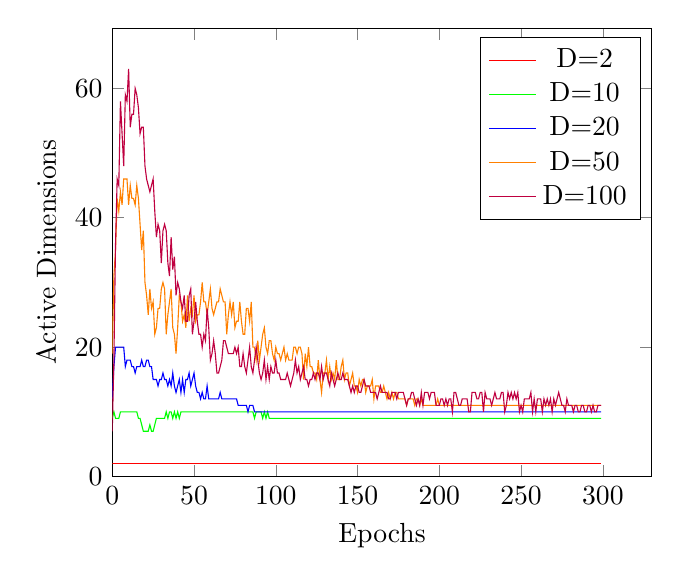
\begin{tikzpicture}\begin{axis}    [% title={Comparison of Dimension Values for Activity},
    xlabel={Epochs},ylabel={Active Dimensions},    xmin=0, xmax=330.0,ymin=0, ymax=69.3,]    \addplot[color=red,]    coordinates {(0,2.0)(1,2.0)(2,2.0)(3,2.0)(4,2.0)(5,2.0)(6,2.0)(7,2.0)(8,2.0)(9,2.0)(10,2.0)(11,2.0)(12,2.0)(13,2.0)(14,2.0)(15,2.0)(16,2.0)(17,2.0)(18,2.0)(19,2.0)(20,2.0)(21,2.0)(22,2.0)(23,2.0)(24,2.0)(25,2.0)(26,2.0)(27,2.0)(28,2.0)(29,2.0)(30,2.0)(31,2.0)(32,2.0)(33,2.0)(34,2.0)(35,2.0)(36,2.0)(37,2.0)(38,2.0)(39,2.0)(40,2.0)(41,2.0)(42,2.0)(43,2.0)(44,2.0)(45,2.0)(46,2.0)(47,2.0)(48,2.0)(49,2.0)(50,2.0)(51,2.0)(52,2.0)(53,2.0)(54,2.0)(55,2.0)(56,2.0)(57,2.0)(58,2.0)(59,2.0)(60,2.0)(61,2.0)(62,2.0)(63,2.0)(64,2.0)(65,2.0)(66,2.0)(67,2.0)(68,2.0)(69,2.0)(70,2.0)(71,2.0)(72,2.0)(73,2.0)(74,2.0)(75,2.0)(76,2.0)(77,2.0)(78,2.0)(79,2.0)(80,2.0)(81,2.0)(82,2.0)(83,2.0)(84,2.0)(85,2.0)(86,2.0)(87,2.0)(88,2.0)(89,2.0)(90,2.0)(91,2.0)(92,2.0)(93,2.0)(94,2.0)(95,2.0)(96,2.0)(97,2.0)(98,2.0)(99,2.0)(100,2.0)(101,2.0)(102,2.0)(103,2.0)(104,2.0)(105,2.0)(106,2.0)(107,2.0)(108,2.0)(109,2.0)(110,2.0)(111,2.0)(112,2.0)(113,2.0)(114,2.0)(115,2.0)(116,2.0)(117,2.0)(118,2.0)(119,2.0)(120,2.0)(121,2.0)(122,2.0)(123,2.0)(124,2.0)(125,2.0)(126,2.0)(127,2.0)(128,2.0)(129,2.0)(130,2.0)(131,2.0)(132,2.0)(133,2.0)(134,2.0)(135,2.0)(136,2.0)(137,2.0)(138,2.0)(139,2.0)(140,2.0)(141,2.0)(142,2.0)(143,2.0)(144,2.0)(145,2.0)(146,2.0)(147,2.0)(148,2.0)(149,2.0)(150,2.0)(151,2.0)(152,2.0)(153,2.0)(154,2.0)(155,2.0)(156,2.0)(157,2.0)(158,2.0)(159,2.0)(160,2.0)(161,2.0)(162,2.0)(163,2.0)(164,2.0)(165,2.0)(166,2.0)(167,2.0)(168,2.0)(169,2.0)(170,2.0)(171,2.0)(172,2.0)(173,2.0)(174,2.0)(175,2.0)(176,2.0)(177,2.0)(178,2.0)(179,2.0)(180,2.0)(181,2.0)(182,2.0)(183,2.0)(184,2.0)(185,2.0)(186,2.0)(187,2.0)(188,2.0)(189,2.0)(190,2.0)(191,2.0)(192,2.0)(193,2.0)(194,2.0)(195,2.0)(196,2.0)(197,2.0)(198,2.0)(199,2.0)(200,2.0)(201,2.0)(202,2.0)(203,2.0)(204,2.0)(205,2.0)(206,2.0)(207,2.0)(208,2.0)(209,2.0)(210,2.0)(211,2.0)(212,2.0)(213,2.0)(214,2.0)(215,2.0)(216,2.0)(217,2.0)(218,2.0)(219,2.0)(220,2.0)(221,2.0)(222,2.0)(223,2.0)(224,2.0)(225,2.0)(226,2.0)(227,2.0)(228,2.0)(229,2.0)(230,2.0)(231,2.0)(232,2.0)(233,2.0)(234,2.0)(235,2.0)(236,2.0)(237,2.0)(238,2.0)(239,2.0)(240,2.0)(241,2.0)(242,2.0)(243,2.0)(244,2.0)(245,2.0)(246,2.0)(247,2.0)(248,2.0)(249,2.0)(250,2.0)(251,2.0)(252,2.0)(253,2.0)(254,2.0)(255,2.0)(256,2.0)(257,2.0)(258,2.0)(259,2.0)(260,2.0)(261,2.0)(262,2.0)(263,2.0)(264,2.0)(265,2.0)(266,2.0)(267,2.0)(268,2.0)(269,2.0)(270,2.0)(271,2.0)(272,2.0)(273,2.0)(274,2.0)(275,2.0)(276,2.0)(277,2.0)(278,2.0)(279,2.0)(280,2.0)(281,2.0)(282,2.0)(283,2.0)(284,2.0)(285,2.0)(286,2.0)(287,2.0)(288,2.0)(289,2.0)(290,2.0)(291,2.0)(292,2.0)(293,2.0)(294,2.0)(295,2.0)(296,2.0)(297,2.0)(298,2.0)(299,2.0)    };    \addplot[color=green,]    coordinates {(0,9.0)(1,10.0)(2,9.0)(3,9.0)(4,9.0)(5,10.0)(6,10.0)(7,10.0)(8,10.0)(9,10.0)(10,10.0)(11,10.0)(12,10.0)(13,10.0)(14,10.0)(15,10.0)(16,9.0)(17,9.0)(18,8.0)(19,7.0)(20,7.0)(21,7.0)(22,7.0)(23,8.0)(24,7.0)(25,7.0)(26,8.0)(27,9.0)(28,9.0)(29,9.0)(30,9.0)(31,9.0)(32,9.0)(33,10.0)(34,9.0)(35,10.0)(36,10.0)(37,9.0)(38,10.0)(39,9.0)(40,10.0)(41,9.0)(42,10.0)(43,10.0)(44,10.0)(45,10.0)(46,10.0)(47,10.0)(48,10.0)(49,10.0)(50,10.0)(51,10.0)(52,10.0)(53,10.0)(54,10.0)(55,10.0)(56,10.0)(57,10.0)(58,10.0)(59,10.0)(60,10.0)(61,10.0)(62,10.0)(63,10.0)(64,10.0)(65,10.0)(66,10.0)(67,10.0)(68,10.0)(69,10.0)(70,10.0)(71,10.0)(72,10.0)(73,10.0)(74,10.0)(75,10.0)(76,10.0)(77,10.0)(78,10.0)(79,10.0)(80,10.0)(81,10.0)(82,10.0)(83,10.0)(84,10.0)(85,10.0)(86,10.0)(87,9.0)(88,10.0)(89,10.0)(90,10.0)(91,10.0)(92,9.0)(93,10.0)(94,9.0)(95,10.0)(96,9.0)(97,9.0)(98,9.0)(99,9.0)(100,9.0)(101,9.0)(102,9.0)(103,9.0)(104,9.0)(105,9.0)(106,9.0)(107,9.0)(108,9.0)(109,9.0)(110,9.0)(111,9.0)(112,9.0)(113,9.0)(114,9.0)(115,9.0)(116,9.0)(117,9.0)(118,9.0)(119,9.0)(120,9.0)(121,9.0)(122,9.0)(123,9.0)(124,9.0)(125,9.0)(126,9.0)(127,9.0)(128,9.0)(129,9.0)(130,9.0)(131,9.0)(132,9.0)(133,9.0)(134,9.0)(135,9.0)(136,9.0)(137,9.0)(138,9.0)(139,9.0)(140,9.0)(141,9.0)(142,9.0)(143,9.0)(144,9.0)(145,9.0)(146,9.0)(147,9.0)(148,9.0)(149,9.0)(150,9.0)(151,9.0)(152,9.0)(153,9.0)(154,9.0)(155,9.0)(156,9.0)(157,9.0)(158,9.0)(159,9.0)(160,9.0)(161,9.0)(162,9.0)(163,9.0)(164,9.0)(165,9.0)(166,9.0)(167,9.0)(168,9.0)(169,9.0)(170,9.0)(171,9.0)(172,9.0)(173,9.0)(174,9.0)(175,9.0)(176,9.0)(177,9.0)(178,9.0)(179,9.0)(180,9.0)(181,9.0)(182,9.0)(183,9.0)(184,9.0)(185,9.0)(186,9.0)(187,9.0)(188,9.0)(189,9.0)(190,9.0)(191,9.0)(192,9.0)(193,9.0)(194,9.0)(195,9.0)(196,9.0)(197,9.0)(198,9.0)(199,9.0)(200,9.0)(201,9.0)(202,9.0)(203,9.0)(204,9.0)(205,9.0)(206,9.0)(207,9.0)(208,9.0)(209,9.0)(210,9.0)(211,9.0)(212,9.0)(213,9.0)(214,9.0)(215,9.0)(216,9.0)(217,9.0)(218,9.0)(219,9.0)(220,9.0)(221,9.0)(222,9.0)(223,9.0)(224,9.0)(225,9.0)(226,9.0)(227,9.0)(228,9.0)(229,9.0)(230,9.0)(231,9.0)(232,9.0)(233,9.0)(234,9.0)(235,9.0)(236,9.0)(237,9.0)(238,9.0)(239,9.0)(240,9.0)(241,9.0)(242,9.0)(243,9.0)(244,9.0)(245,9.0)(246,9.0)(247,9.0)(248,9.0)(249,9.0)(250,9.0)(251,9.0)(252,9.0)(253,9.0)(254,9.0)(255,9.0)(256,9.0)(257,9.0)(258,9.0)(259,9.0)(260,9.0)(261,9.0)(262,9.0)(263,9.0)(264,9.0)(265,9.0)(266,9.0)(267,9.0)(268,9.0)(269,9.0)(270,9.0)(271,9.0)(272,9.0)(273,9.0)(274,9.0)(275,9.0)(276,9.0)(277,9.0)(278,9.0)(279,9.0)(280,9.0)(281,9.0)(282,9.0)(283,9.0)(284,9.0)(285,9.0)(286,9.0)(287,9.0)(288,9.0)(289,9.0)(290,9.0)(291,9.0)(292,9.0)(293,9.0)(294,9.0)(295,9.0)(296,9.0)(297,9.0)(298,9.0)(299,9.0)    };    \addplot[color=blue,]    coordinates {(0,12.0)(1,17.0)(2,20.0)(3,20.0)(4,20.0)(5,20.0)(6,20.0)(7,20.0)(8,17.0)(9,18.0)(10,18.0)(11,18.0)(12,17.0)(13,17.0)(14,16.0)(15,17.0)(16,17.0)(17,17.0)(18,18.0)(19,17.0)(20,17.0)(21,18.0)(22,18.0)(23,17.0)(24,17.0)(25,15.0)(26,15.0)(27,15.0)(28,14.0)(29,15.0)(30,15.0)(31,16.0)(32,15.0)(33,15.0)(34,14.0)(35,15.0)(36,14.0)(37,16.0)(38,14.0)(39,13.0)(40,14.0)(41,15.0)(42,13.0)(43,15.0)(44,13.0)(45,15.0)(46,15.0)(47,16.0)(48,14.0)(49,15.0)(50,16.0)(51,14.0)(52,13.0)(53,13.0)(54,12.0)(55,13.0)(56,12.0)(57,12.0)(58,14.0)(59,12.0)(60,12.0)(61,12.0)(62,12.0)(63,12.0)(64,12.0)(65,12.0)(66,13.0)(67,12.0)(68,12.0)(69,12.0)(70,12.0)(71,12.0)(72,12.0)(73,12.0)(74,12.0)(75,12.0)(76,12.0)(77,11.0)(78,11.0)(79,11.0)(80,11.0)(81,11.0)(82,11.0)(83,10.0)(84,11.0)(85,11.0)(86,11.0)(87,10.0)(88,10.0)(89,10.0)(90,10.0)(91,10.0)(92,10.0)(93,10.0)(94,10.0)(95,10.0)(96,10.0)(97,10.0)(98,10.0)(99,10.0)(100,10.0)(101,10.0)(102,10.0)(103,10.0)(104,10.0)(105,10.0)(106,10.0)(107,10.0)(108,10.0)(109,10.0)(110,10.0)(111,10.0)(112,10.0)(113,10.0)(114,10.0)(115,10.0)(116,10.0)(117,10.0)(118,10.0)(119,10.0)(120,10.0)(121,10.0)(122,10.0)(123,10.0)(124,10.0)(125,10.0)(126,10.0)(127,10.0)(128,10.0)(129,10.0)(130,10.0)(131,10.0)(132,10.0)(133,10.0)(134,10.0)(135,10.0)(136,10.0)(137,10.0)(138,10.0)(139,10.0)(140,10.0)(141,10.0)(142,10.0)(143,10.0)(144,10.0)(145,10.0)(146,10.0)(147,10.0)(148,10.0)(149,10.0)(150,10.0)(151,10.0)(152,10.0)(153,10.0)(154,10.0)(155,10.0)(156,10.0)(157,10.0)(158,10.0)(159,10.0)(160,10.0)(161,10.0)(162,10.0)(163,10.0)(164,10.0)(165,10.0)(166,10.0)(167,10.0)(168,10.0)(169,10.0)(170,10.0)(171,10.0)(172,10.0)(173,10.0)(174,10.0)(175,10.0)(176,10.0)(177,10.0)(178,10.0)(179,10.0)(180,10.0)(181,10.0)(182,10.0)(183,10.0)(184,10.0)(185,10.0)(186,10.0)(187,10.0)(188,10.0)(189,10.0)(190,10.0)(191,10.0)(192,10.0)(193,10.0)(194,10.0)(195,10.0)(196,10.0)(197,10.0)(198,10.0)(199,10.0)(200,10.0)(201,10.0)(202,10.0)(203,10.0)(204,10.0)(205,10.0)(206,10.0)(207,10.0)(208,10.0)(209,10.0)(210,10.0)(211,10.0)(212,10.0)(213,10.0)(214,10.0)(215,10.0)(216,10.0)(217,10.0)(218,10.0)(219,10.0)(220,10.0)(221,10.0)(222,10.0)(223,10.0)(224,10.0)(225,10.0)(226,10.0)(227,10.0)(228,10.0)(229,10.0)(230,10.0)(231,10.0)(232,10.0)(233,10.0)(234,10.0)(235,10.0)(236,10.0)(237,10.0)(238,10.0)(239,10.0)(240,10.0)(241,10.0)(242,10.0)(243,10.0)(244,10.0)(245,10.0)(246,10.0)(247,10.0)(248,10.0)(249,10.0)(250,10.0)(251,10.0)(252,10.0)(253,10.0)(254,10.0)(255,10.0)(256,10.0)(257,10.0)(258,10.0)(259,10.0)(260,10.0)(261,10.0)(262,10.0)(263,10.0)(264,10.0)(265,10.0)(266,10.0)(267,10.0)(268,10.0)(269,10.0)(270,10.0)(271,10.0)(272,10.0)(273,10.0)(274,10.0)(275,10.0)(276,10.0)(277,10.0)(278,10.0)(279,10.0)(280,10.0)(281,10.0)(282,10.0)(283,10.0)(284,10.0)(285,10.0)(286,10.0)(287,10.0)(288,10.0)(289,10.0)(290,10.0)(291,10.0)(292,10.0)(293,10.0)(294,10.0)(295,10.0)(296,10.0)(297,10.0)(298,10.0)(299,10.0)    };    \addplot[color=orange,]    coordinates {(0,19.0)(1,31.0)(2,35.0)(3,43.0)(4,41.0)(5,44.0)(6,42.0)(7,46.0)(8,46.0)(9,46.0)(10,42.0)(11,45.0)(12,43.0)(13,43.0)(14,42.0)(15,45.0)(16,43.0)(17,39.0)(18,35.0)(19,38.0)(20,30.0)(21,28.0)(22,25.0)(23,29.0)(24,26.0)(25,27.0)(26,22.0)(27,23.0)(28,26.0)(29,26.0)(30,29.0)(31,30.0)(32,29.0)(33,22.0)(34,25.0)(35,27.0)(36,29.0)(37,23.0)(38,22.0)(39,19.0)(40,23.0)(41,28.0)(42,27.0)(43,24.0)(44,25.0)(45,23.0)(46,28.0)(47,24.0)(48,26.0)(49,25.0)(50,28.0)(51,24.0)(52,25.0)(53,25.0)(54,27.0)(55,30.0)(56,27.0)(57,27.0)(58,25.0)(59,27.0)(60,29.0)(61,26.0)(62,25.0)(63,26.0)(64,27.0)(65,27.0)(66,29.0)(67,28.0)(68,27.0)(69,27.0)(70,22.0)(71,25.0)(72,27.0)(73,25.0)(74,27.0)(75,23.0)(76,24.0)(77,24.0)(78,27.0)(79,24.0)(80,22.0)(81,22.0)(82,26.0)(83,26.0)(84,24.0)(85,27.0)(86,20.0)(87,20.0)(88,18.0)(89,21.0)(90,18.0)(91,20.0)(92,22.0)(93,23.0)(94,20.0)(95,19.0)(96,21.0)(97,21.0)(98,19.0)(99,18.0)(100,20.0)(101,19.0)(102,19.0)(103,18.0)(104,19.0)(105,20.0)(106,18.0)(107,19.0)(108,18.0)(109,18.0)(110,18.0)(111,20.0)(112,20.0)(113,19.0)(114,20.0)(115,20.0)(116,19.0)(117,15.0)(118,19.0)(119,17.0)(120,20.0)(121,17.0)(122,17.0)(123,16.0)(124,16.0)(125,15.0)(126,18.0)(127,15.0)(128,13.0)(129,16.0)(130,16.0)(131,18.0)(132,15.0)(133,17.0)(134,15.0)(135,16.0)(136,15.0)(137,18.0)(138,15.0)(139,15.0)(140,17.0)(141,18.0)(142,15.0)(143,16.0)(144,16.0)(145,14.0)(146,15.0)(147,16.0)(148,14.0)(149,14.0)(150,13.0)(151,15.0)(152,14.0)(153,15.0)(154,15.0)(155,13.0)(156,14.0)(157,14.0)(158,14.0)(159,15.0)(160,12.0)(161,14.0)(162,14.0)(163,14.0)(164,13.0)(165,13.0)(166,14.0)(167,13.0)(168,12.0)(169,13.0)(170,12.0)(171,13.0)(172,12.0)(173,13.0)(174,13.0)(175,12.0)(176,12.0)(177,12.0)(178,12.0)(179,12.0)(180,11.0)(181,12.0)(182,12.0)(183,12.0)(184,12.0)(185,11.0)(186,12.0)(187,12.0)(188,11.0)(189,12.0)(190,11.0)(191,11.0)(192,11.0)(193,11.0)(194,11.0)(195,11.0)(196,11.0)(197,11.0)(198,11.0)(199,12.0)(200,11.0)(201,11.0)(202,11.0)(203,11.0)(204,11.0)(205,11.0)(206,11.0)(207,11.0)(208,11.0)(209,11.0)(210,11.0)(211,11.0)(212,11.0)(213,11.0)(214,11.0)(215,11.0)(216,11.0)(217,11.0)(218,11.0)(219,11.0)(220,11.0)(221,11.0)(222,11.0)(223,11.0)(224,11.0)(225,11.0)(226,11.0)(227,11.0)(228,11.0)(229,11.0)(230,11.0)(231,11.0)(232,11.0)(233,11.0)(234,11.0)(235,11.0)(236,11.0)(237,11.0)(238,11.0)(239,11.0)(240,11.0)(241,11.0)(242,11.0)(243,11.0)(244,11.0)(245,11.0)(246,11.0)(247,11.0)(248,11.0)(249,11.0)(250,11.0)(251,11.0)(252,11.0)(253,11.0)(254,11.0)(255,11.0)(256,11.0)(257,11.0)(258,11.0)(259,11.0)(260,11.0)(261,11.0)(262,11.0)(263,11.0)(264,11.0)(265,11.0)(266,11.0)(267,11.0)(268,11.0)(269,11.0)(270,11.0)(271,11.0)(272,11.0)(273,11.0)(274,11.0)(275,11.0)(276,11.0)(277,11.0)(278,11.0)(279,11.0)(280,11.0)(281,11.0)(282,11.0)(283,11.0)(284,11.0)(285,11.0)(286,11.0)(287,11.0)(288,11.0)(289,11.0)(290,11.0)(291,11.0)(292,11.0)(293,11.0)(294,11.0)(295,11.0)(296,11.0)(297,11.0)(298,11.0)(299,11.0)    };    \addplot[color=purple,]    coordinates {(0,7.0)(1,18.0)(2,36.0)(3,46.0)(4,45.0)(5,58.0)(6,53.0)(7,48.0)(8,59.0)(9,58.0)(10,63.0)(11,54.0)(12,56.0)(13,56.0)(14,60.0)(15,59.0)(16,57.0)(17,53.0)(18,54.0)(19,54.0)(20,48.0)(21,46.0)(22,45.0)(23,44.0)(24,45.0)(25,46.0)(26,41.0)(27,37.0)(28,39.0)(29,38.0)(30,33.0)(31,38.0)(32,39.0)(33,38.0)(34,33.0)(35,31.0)(36,37.0)(37,32.0)(38,34.0)(39,28.0)(40,30.0)(41,29.0)(42,27.0)(43,26.0)(44,28.0)(45,24.0)(46,24.0)(47,28.0)(48,29.0)(49,22.0)(50,24.0)(51,27.0)(52,24.0)(53,22.0)(54,22.0)(55,20.0)(56,22.0)(57,21.0)(58,26.0)(59,23.0)(60,18.0)(61,19.0)(62,21.0)(63,19.0)(64,16.0)(65,16.0)(66,17.0)(67,18.0)(68,21.0)(69,21.0)(70,20.0)(71,19.0)(72,19.0)(73,19.0)(74,19.0)(75,20.0)(76,19.0)(77,20.0)(78,17.0)(79,17.0)(80,19.0)(81,17.0)(82,16.0)(83,18.0)(84,20.0)(85,17.0)(86,16.0)(87,18.0)(88,20.0)(89,18.0)(90,16.0)(91,15.0)(92,16.0)(93,18.0)(94,15.0)(95,17.0)(96,15.0)(97,17.0)(98,16.0)(99,16.0)(100,18.0)(101,16.0)(102,16.0)(103,15.0)(104,15.0)(105,15.0)(106,15.0)(107,16.0)(108,15.0)(109,14.0)(110,15.0)(111,16.0)(112,18.0)(113,16.0)(114,17.0)(115,15.0)(116,16.0)(117,17.0)(118,15.0)(119,15.0)(120,14.0)(121,15.0)(122,15.0)(123,16.0)(124,15.0)(125,16.0)(126,16.0)(127,15.0)(128,17.0)(129,15.0)(130,16.0)(131,16.0)(132,15.0)(133,14.0)(134,16.0)(135,15.0)(136,14.0)(137,15.0)(138,16.0)(139,15.0)(140,15.0)(141,16.0)(142,15.0)(143,15.0)(144,15.0)(145,14.0)(146,13.0)(147,14.0)(148,13.0)(149,14.0)(150,14.0)(151,13.0)(152,13.0)(153,14.0)(154,15.0)(155,14.0)(156,14.0)(157,14.0)(158,13.0)(159,13.0)(160,13.0)(161,13.0)(162,12.0)(163,13.0)(164,14.0)(165,13.0)(166,13.0)(167,13.0)(168,13.0)(169,12.0)(170,12.0)(171,13.0)(172,13.0)(173,13.0)(174,12.0)(175,13.0)(176,13.0)(177,13.0)(178,13.0)(179,12.0)(180,11.0)(181,12.0)(182,12.0)(183,13.0)(184,13.0)(185,12.0)(186,11.0)(187,12.0)(188,11.0)(189,13.0)(190,11.0)(191,13.0)(192,13.0)(193,13.0)(194,12.0)(195,13.0)(196,13.0)(197,13.0)(198,11.0)(199,11.0)(200,11.0)(201,12.0)(202,12.0)(203,11.0)(204,12.0)(205,11.0)(206,12.0)(207,12.0)(208,10.0)(209,13.0)(210,13.0)(211,12.0)(212,11.0)(213,11.0)(214,12.0)(215,12.0)(216,12.0)(217,12.0)(218,10.0)(219,10.0)(220,13.0)(221,13.0)(222,13.0)(223,12.0)(224,12.0)(225,13.0)(226,13.0)(227,10.0)(228,13.0)(229,12.0)(230,12.0)(231,12.0)(232,11.0)(233,12.0)(234,13.0)(235,12.0)(236,12.0)(237,12.0)(238,13.0)(239,13.0)(240,10.0)(241,11.0)(242,13.0)(243,12.0)(244,13.0)(245,12.0)(246,13.0)(247,12.0)(248,13.0)(249,10.0)(250,11.0)(251,10.0)(252,12.0)(253,12.0)(254,12.0)(255,12.0)(256,13.0)(257,10.0)(258,12.0)(259,10.0)(260,12.0)(261,12.0)(262,12.0)(263,10.0)(264,12.0)(265,11.0)(266,12.0)(267,11.0)(268,12.0)(269,10.0)(270,12.0)(271,11.0)(272,12.0)(273,13.0)(274,12.0)(275,11.0)(276,11.0)(277,10.0)(278,12.0)(279,11.0)(280,11.0)(281,11.0)(282,10.0)(283,11.0)(284,11.0)(285,10.0)(286,10.0)(287,11.0)(288,11.0)(289,10.0)(290,10.0)(291,11.0)(292,11.0)(293,10.0)(294,11.0)(295,10.0)(296,10.0)(297,11.0)(298,11.0)(299,11.0)    };    \legend{D=2,D=10,D=20,D=50,D=100,}\end{axis}\end{tikzpicture}\\
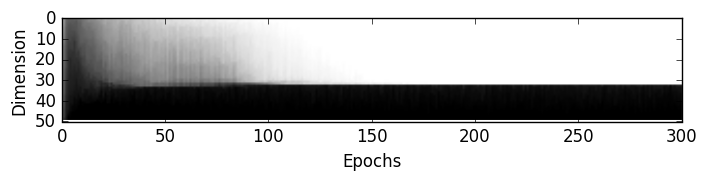
\includegraphics[scale=0.75]{{../img/trial.50.1.0.0.0.0.Berno}.png}\\
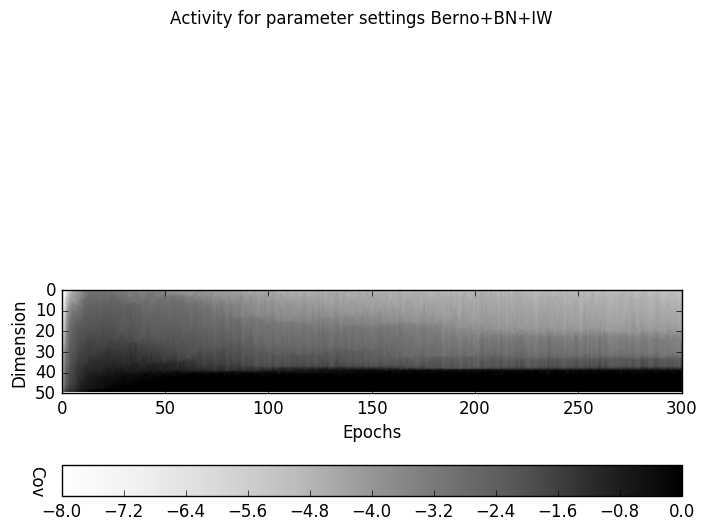
\includegraphics[scale=0.75]{{../img/trial.50.1.0.1.0.1.Berno+BN+IW}.png}\\
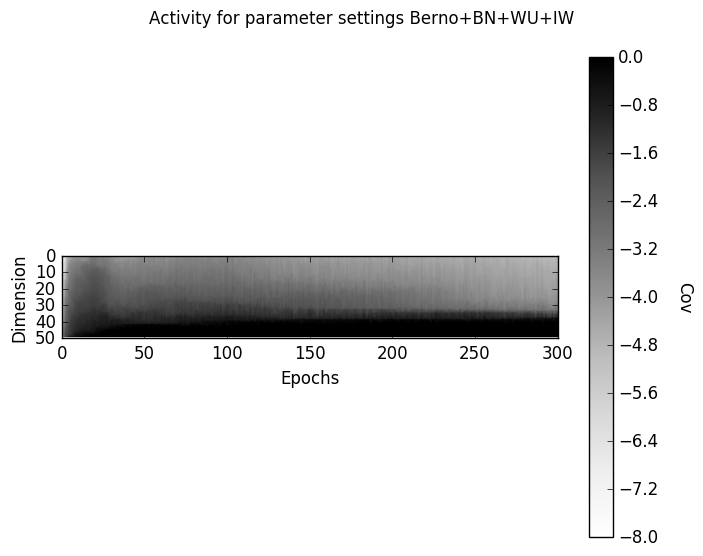
\includegraphics[scale=0.75]{{../img/trial.50.1.0.1.1.1.Berno+BN+WU+IW}.png}\\
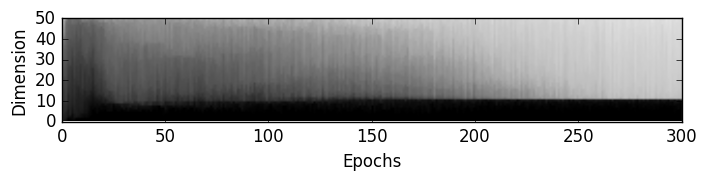
\includegraphics[scale=0.75]{{../img/trial.50.1.0.0.0.1.Berno+IW}.png}\\
\end{document}
